\documentclass[galley,usenatbib]{mn2e}
%\documentclass[twocolumn,galley]{mn2e}
%\documentclass[onecolumn,galley,draft]{mn2e}
\usepackage{myaasmacros}
\usepackage{mathrsfs}
\usepackage{amsmath}
\usepackage{graphicx}
\usepackage{ulem} % Only necessary for striking out TODO items see \sout

\def\newblock{\hskip .11em plus .33em minus .07em}

\newcommand{\Glass}{{\sc Glass}}
\newcommand{\PixeLens}{{\sc PixeLens}}
\newcommand{\Rmap}{\ensuremath{R_\mathrm{map}}}
\newcommand{\Rpix}{\ensuremath{R_\mathrm{pix}}}
\newcommand{\M}{\ensuremath{\mathscr{M}}}
\newcommand{\E}{\ensuremath{\mathscr{E}}}
\newcommand{\eps}{\ensuremath{\varepsilon}}

\newcommand{\Eavg}{\ensuremath{\langle \E \rangle}}

\newcommand{\kpc}{\ensuremath{\mathrm{kpc}}}
\newcommand{\Msun}{\ensuremath{\mathrm{M}_\odot}}
\newcommand{\tabref}[1] {Table~\ref{#1}}
\newcommand{\figref}[1] {Figure~\ref{#1}}
\newcommand{\eqnref}[1] {Eq.~(\ref{#1})}
\newcommand{\secref}[1] {\S\ref{#1}}
\newcommand{\appref}[1] {Appendix~\ref{#1}}
\newcommand{\e}[1]{\ensuremath{\times 10^{#1}}}
\renewcommand{\vec}[1]{\ensuremath{\boldsymbol{#1}}}

\newcommand{\mockAA}{{\sc Ssteep-DMshallow}}
\newcommand{\mockAC}{{\sc Ssteep-DMsteep}}
\newcommand{\mockBB}{{\sc Ssteep-DMshallow}}
\newcommand{\mockBC}{{\sc Ssteep-DMsteep}}

% From aastex.cls
\newcommand\plotone[1]{%
 \centering
 \leavevmode
 \includegraphics[width={\columnwidth}]{#1}%
}%
\newcommand\plottwo[2]{{%
 \centering
 \leavevmode
 \columnwidth=.45\columnwidth
 \includegraphics[width={\columnwidth}]{#1}%
 \hfil
 \includegraphics[width={\columnwidth}]{#2}%
}}%
\newcommand\plotthree[3]{{%
 \centering
 \leavevmode
 \columnwidth=.30\textwidth
 \includegraphics[width={\columnwidth}]{#1}%
 \hfil
 \includegraphics[width={\columnwidth}]{#2}%
 \hfil
 \includegraphics[width={\columnwidth}]{#3}%
}}%


\title[\Glass]{Gravitational Lens Recovery with \Glass: How to measure the mass profile and shape of a lens}
\author{%
Jonathan P. Coles 
\and 
Justin I. Read
\and 
Prasenjit Saha 
}

\begin{document}
\maketitle

\begin{abstract}
We use a new non-parametric gravitational -- \Glass -- to determine what quality of data (strong lensing, stellar kinematics, and/or stellar masses) are required to measure the circularly averaged mass profile of a lens and its shape. \Glass\ uses an under-constrained adaptive grid of mass pixels to model the lens, searching through thousands of models to marginalise over model uncertainties. Our key findings are as follows: (i) for pure lens data, multiple sources with wide redshift separation give the strongest constraints as this breaks the well-known mass-sheet or steepness degeneracy; (ii) a single quad with time delays also performs well, giving a good recovery of both the mass profile and its shape; (iii) stellar masses -- for lenses where the stars dominate the central potential -- can also break the steepness degeneracy, giving a recovery almost as good as having time delay data or multiple source redshifts; (iv) stellar kinematics are similarly powerful if the data extend beyond the half light radius of the stars $r \gg r_{1/2}$ (required to integrate out the effect of the unknown velocity anisotropy, $\beta(r)$); and (v) if the lensing data already probe the mass profile over the region $r \sim r_{1/2}$, then stellar kinematic data can be used to probe $\beta(r)$ -- an interesting dynamic quantity in its own right. Where information on the mass distribution from lensing and other probes becomes redundant, this opens up the possibility of using strong lensing to constrain cosmological models. We will study this, and present the first results from \Glass\ applied to real data, in forthcoming papers.
\end{abstract}

%(Linear constraints are applied simultaneously with the lens constraints; non-linear constraints are applied in post-processing, with models accepted or rejected based on their likelihood.) 
%These are quantities of key interest for probing the dark matter distribution in galaxies and galaxy clusters to test galaxy formation models and cosmology.

\section{Introduction}\label{sec:intro} %-----------------------------------------------------

Strong gravitational lenses are rare.  The reason is that the line of
sight to a light source in the universe rarely goes through a region
such that the projected density in its sky neighbourhood exceeds the
critical density to produce multiple images.  To date, some $\sim400$
strong lenses are known,\footnote{See {\tt http://www.masterlens.org}
  for a catalogue.}  but this number is expected to increase to
several thousand over the next ten years.  The optimism derives from
new and upcoming surveys, both
ground-based\footnote{http://pan-starrs.ifa.hawaii.edu}$^{\rm,}$\footnote{http://www.darkenergysurvey.org}
and spacecraft,\footnote{http://www.euclid-ec.org} together with a
community of citizen-science volunteers examining the image data for
candidates.\footnote{http://spacewarps.org}

Since lensing depends only on gravity, strong lenses are a rather
unique window on dark matter, and indirectly on the cosmological model
as well, and hence the thousands of to-be-discovered lenses are
eagerly awaited \citep{2010CQGra..27w3001B,2012arXiv1206.1225A}.
Extracting results from lensing, however, will require modelling, and
it is towards that goal that the present work is directed.

To see why lens modelling is of crucial importance, let us recall the
essential quantities that appear in lensing.  First we have the
distances: let $D_L$, $D_S$, $D_{LS}$ be the angular-diameter
distances to the lens, source, and from lens to source; there are all
strictly $\propto c/H_0$.  Typically
\begin{equation}
D_L \approx z \frac c{H_0}\ \hbox{and}\ \frac{D_S}{D_{LS}} \sim 1.
\end{equation}
For multiple images the sky-projected density must exceed the critical
density of $D_S/D_{LS}$ times
\begin{equation}
\Sigma_L = \frac{c^2}{4\pi G D_L} \sim \frac{1\rm\,kg\,m^{-2}}{z_L}
\end{equation}
in some region.  The separation between the lensed images is of order
the Einstein radius $\theta_E$.  The image separation is related to
the mass by
\begin{equation}
\theta_E \sim \frac{R_G}{D_L} \frac{D_{LS}}{D_S}
\end{equation}
where $R_G$ is the gravitational radius $GM/c^2$.  If the source is a
quasar or otherwise rapidly variable, a time delay is the variability
will be present
\begin{equation}
\Delta t \sim R_G/c \,.
\end{equation}
So in principle, one can not only measure the mass of the lens, one
can use the dependence on the cosmology-dependent $D$ factors to
extract the cosmological model and all its parameters.
\cite{1937ApJ....86..217Z} drew attention to the former, and
\cite{1964MNRAS.128..307R,1966MNRAS.132..101R} pointed out the latter,
all long before lenses were discovered.  The difficulty became
apparent soon after the discovery of the first lens by
\cite{1979Natur.279..381W}.  In the first ever paper on lens
modelling, \cite{1981ApJ...244..736Y} found that many plausible mass
distributions could reproduce the data.

% Simple parametric models are usually robust on qualitative features,
% but other aspects can be very model-dependent
% \citep[cf.~][]{2003AJ....125.2769S}.  For example, for lensed
% quasars, there may be several models all providing excellent fits to
% the image data but disagreeing on the expected time delays, but they
% almost always agree about the {\em order\/} of time delays. Thus, a
% simple model provides valuable physical insight, but as data quality
% improves and the questions we ask of these data become more refined,
% it is important to re-assess the impact of our model assumptions.
% The key advantages of non-parametric modelling are that we can: (i)
% explore model degeneracies and marginalise over them; and (ii) we
% can determine what type and quality of data are required to measure
% parameters of interest.

\cite{1981ApJ...244..736Y} were remarkably prescient about the
subsequent development of lens modelling.  First, the introduced the
technique of choosing a parametric form for the lensing mass and then
fitting for the parameters, which is still the most common strategy
\citep[see for example][]{2010GReGr..42.2151K,2011A&ARv..19...47K}.
Second, they pointed out the non-uniqueness of lens models, or lensing
degeneracies.  Third, they suggested combining lensing data with
stellar kinematics and X-rays, to reduce the effect of the
degeneracies.  Later work, as well as following up these suggestions,
has introduced some ideas.  Four of these are important in the present
work.
\begin{itemize}
\item In free-form models, there is no specified parametric form for
  the mass distribution.  There are still assumptions (or priors) on
  the mass distribution, such as smoothness or being centrally
  concentrated
  \citep{1997MNRAS.292..148S,2005MNRAS.360..477D,2010ApJ...723.1678C}
  but these are much less restrictive than parametric forms.
  \cite{2006MNRAS.367.1209L} implemented a particular elegant prior,
  which is that the mass distribution must be non-negative and no
  extra images are produced.  Free-form are more commonly used with
  cluster lenses \citep{2009ApJ...690..154S,2013arXiv1304.2393S}, but
  can be used with galaxy lenses as well, where their less restrictive
  assumptions can be important.  For example, in time-delay galaxy
  lenses parametric models led to tensions with the Hubble parameter
  $H_0$ \citep[e.g.][]{2002astro.ph..4043K,2002ApJ...578...25K}, but
  the less restrictive assumptions of free-form models resolved these
  tensions \citep{2007ApJ...667..645R}.
\item Model ensembles, exploring a diverse range of possible mass
  distributions that nonetheless all fit the data, are a way of
  cambating the non-uniqueness of models.  Model ensembles are
  possible in parametric models \citep{1999AJ....118...14B} but are
  more common in free-form models
  \citep{2000AJ....119..439W,2009ApJ...690..154S,2012MNRAS.425.3077L}.
\item Stellar kinematics has played a role in many modelling
  techniques.  The underlying reason is the virial theorem, which
  relates the line of sight velocity dispersion to the Einstein radius
  as
\begin{equation}
  \frac{\langle v^2_{\rm los}\rangle}{c^2} \approx
  \frac{\theta_E}{6\pi} \frac{D_S}{D_{LS}}
\end{equation}
  with the relation becoming exact for isothermal lenses.  The use of
  two-dimensional kinematics by \cite{2011MNRAS.415.2215B} is
  especially interesting.
\item The stellar mass in a lens can be inferred from photometry and
  compared with the total mass
  \citep{2005ApJ...623L...5F,2008MNRAS.383..857F,2011ApJ...740...97L}.
  Since the inferred stellar mass does depend on the assumed IMF,
  lenses in which stellar mass dominates can be used to derive upper
  bounds on the stellar $M/L$ \cite{2010MNRAS.409L..30F}. Lower bounds
  on stellar $M/L$ have also been claimed \citep{2013MNRAS.428.3183D}
  but these require upper-bound assumptions about the dark-matter
  profile.
\item Testing modelling strategies to see how well they recover
  simulated lenses is increasingly recognized as essential.  Simple
  blind tests have appeared in earlier work \citep[for example, Figure
    2 in][]{2000AJ....119..439W}, but more recently, test against
  dynamically simulated galaxies are favoured
  \citep{2007ApJ...667..645R,2009MNRAS.393.1114B}.
\end{itemize}
There are also more modelling ideas in the literature.  One is to use
X-ray intensity and temperature profiles as a mass constraint
\citep[such as in][]{2013ApJ...765...25N}.  Another idea is to model
multiple lenses simultaneously, with one or more cosmological
parameters variable but shared between the lenses.  This strategy has
been used to constrain $H_0$ from time delays
\citep{2006ApJ...652L...5S,2008ApJ...679...17C,2010ApJ...712.1378P}.
In principle, cosmological parameters could be constrained even from a
single lens.  Some models have attempted this
\citep{2010Sci...329..924J,2013arXiv1306.4732S} starting from a prior
based on the values and uncertainties from the CMB; tests of this
technique simulated lenses are still awaited, in order to see how far
the results depend on the model assumptions.

In this paper, we use a new program --- \Glass\ --- to determine what
combination of lensing, stellar mass, and stellar kinematic
constraints best constrain the projected mass profile and shape of a
gravitational lens.  The compute-intensive core of \Glass\ is a
parallel implementation of the high-dimensional sampling algorithm
from \cite{2012MNRAS.425.3077L}.  Around that core, \Glass\ has
extensible code (in software terminology, a framework) in Python,
encoding the lens equation, a basis and priors for the mass
distribution, and various post-processing and visualisation modules.  \Glass\
is described in \secref{sec:glass}.  In \secref{sec:theory} before that we
review the elements of lensing theory, stellar population synthesis, and
stellar dynamics we will need.

In \secref{sec:mockdata}, we describe our mock data.

In \secref{sec:results}, we present our results from applying \Glass\ to
these mock data.


\section{Formulation}\label{sec:theory}

\subsection{Lensing essentials}\label{sec:lensing_basic}

We follow \cite{1986ApJ...310..568B} with minor differences in notation.

The lens equation
\begin{equation}
\begin{aligned}
\vec\beta &= \vec\theta - \frac{D_{LS}}{D_S}\vec\alpha(\vec\theta) \\
\vec\alpha(\vec\theta) &= \frac{4G}{c^2D_L} \int \Sigma(\vec\theta')
                          \frac{(\vec\theta - \vec\theta')}
                          {\ |\vec\theta - \vec\theta'|^2} \, d^2\vec\theta'
\end{aligned}
\label{eqn:lens_equation}
\end{equation}
maps an observed image position $\vec\theta$ to a source position
$\vec\beta$.  The lens can then be thought of as a projected surface
density $\Sigma$ which diverts the path of a photon instantaneously
through the bending angle $\vec\alpha$.  The $D$ factors, as in the previous section, are angular
diameter distances, which depend on the particular choice of cosmological
parameters $\Omega$:
\begin{equation}
D_{LS} = \frac c{H_0} \frac{1+z_S}{1+z_L} \int_{z_L}^{z_S}
                      \frac{dz}{\sqrt{\Omega_m(1+z)^3 + \Omega_\Lambda}}
\end{equation}
One way to understand the lens equation is via Fermat's principle. We
can think of light as travelling only along extremum paths where
lensed images occur. Such paths occur at
the extrema of the photon {\it arrival time\/} $t(\vec\theta)$
that depends on the geometric path the photon takes and the general
relativistic gravitational time dilation due to a thin lens at
redshift $z_L$.
\begin{equation}
\begin{aligned}
\frac{ct(\vec\theta)}{(1+z_L)D_{L}}
&= {\textstyle\frac12} |\vec\theta - \vec\beta|^2
   \times \frac{D_{S}}{D_{LS}} \\
&- \frac{4GD_L}{c^2}
   \int \Sigma(\vec\theta') \ln |\vec\theta-\vec\theta'| \, d^2\vec\theta'
\label{full arrival time}
\end{aligned}
\end{equation}
The time here has been scaled to make it dimensionless.  We can make
the density dimensionless as well, by introducing
\begin{equation}
\kappa(\vec\theta) \equiv \frac{\Sigma(\vec\theta)}{\Sigma_L}
\end{equation}
and hence rewrite \eqnref{full arrival time} as
\begin{equation}
\tau(\vec\theta) = {\textstyle\frac12} |\vec\theta - \vec\beta|^2
                   \times \frac{D_{S}}{D_{LS}}
                 - \frac1\pi \int \kappa (\vec\theta')
                   \ln|\vec\theta - \vec\theta'| d^2\vec\theta'
\label{arrival time}
\end{equation}
The scaled arrival time $\tau$ is like a solid angle.  It is of order
the area (in steradians) of the full lensing system --- the expression
$\sim|\vec\theta - \vec\beta|^2$ is of order the image-separation
squared, and the other terms are of similar size.  For this reason, is
convenient to measure $\tau$ in arcsec$^{2}$.

Lensing observations provide information only at $\vec\theta$ where
there are images.  Hence, the arrival-time surface $\tau(\vec\theta)$
is not itself observable.  Its usefulness lies in that observables can
be derived from it.  Thus an image observed at $\vec\theta_1$ implies
that $\nabla\tau(\vec\theta_1)=0$.  A measurement of time delays
between images at $\theta_1$ and $\theta_1$ implies that
$t(\vec\theta_1)-t(\vec\theta_2)$ is known.  Interestingly, both these
types of observations give contraints that are linear in $\kappa$ and
$\vec\beta$.

The rather complicated dependence of lensing observables on the mass
distribution $\kappa(\vec\theta)$ has an important consequence: very
different mass distributions can result in similar observables.  This
is the phenomenon of lensing degeneracies.  While the non-uniqueness
of lens models noted by \cite{1981ApJ...244..736Y} already hinted at
degeneracies, their existence was first derived by
\cite{1985ApJ...289L...1F}.  The most important is the so-called
mass-sheet degeneracy, which is that image positions remain invariant
if the $D_S/D_{LS} - \kappa(\vec\theta)$ are each multiplied by an
arbitrary constant.  This amounts to multiplying the arrival-time
surface by a constant factor.  In fact there are infinitely many
degeneracies \citep{2000AJ....120.1654S} because any transformation of
the arrival-time surface away from the images has no effect on the
lensing observables.  In particular, there are degeneracies that
involve the shape of the mass distribution
\citep{2006ApJ...653..936S,2013arXiv1306.4675S}.  Degeneracies tend to
be suppressed if there are sources at very different redshifts or
`redshift contrast' \citep{1998AJ....116.1541A,2009ApJ...690..154S},
because the presence of different factors of $D_S/D_{LS}$ in the image
plane makes it more difficult to change the mass distribution and the
arrival-time surface without affecting the lensing observables.  But
degeneracies are still present with multiple source redshifts.
\citep{2008MNRAS.386..307L}.


% The only lensing observables from \eqnref{arrival time} are the
% image positions. However, if the source object is variable then the
% observed light curves of each image will be identical but shifted in
% time due to the different photon path lengths.  The time difference
% between identical portions of the light curves is called the time
% delay $\Delta t$ between images.  Using \eqnref{tau} the time delay
% $\Delta t_{21}$ between two images $\vec\theta_1$ and
% $\vec\theta_2$, where $\vec\theta_2$ arrives after $\vec\theta_1$,
% is $\Delta t_{21} = \Delta \tau_{21}(1+z_L)d_L / \zeta$. If $\beta$
% and $\kappa_\infty$ could be known exactly this would allow one to
% precisely infer the angular diameter distance to the lens and thus
% -- via a cosmological model -- the Hubble constant. However, the
% source position is not observable and the density distribution is
% highly degenerate.

% \subsection{Degeneracies}\label{sec:degen}
%
% The trouble with solving the lens equation for the mass distribution is that the solutions are not unique. To see why, it is instructive to simplify \eqnref{eqn:lens_equation} for a circularly symmetric lens: 
%
% \begin{equation}
% \vec\beta = \vec\theta - \frac{\theta_E^2}{\theta^2}\vec\theta
% \label{eqn:lens_equation_circ}
% \end{equation}
%
% where $\theta = |\vec\theta|$, $\theta_E^2 = \frac{D_{LS}}{D_S D_L} \frac{4 GM(<\theta)}{c^2}$ is the Einstein radius, and $M(<\theta)$ is the mass enclosed within the images. 

% For on-axis sources (\vec\beta\ = \vec0), the images split into a degenerate Einstein ring with $\theta = \theta_E$. Even in this situation of maximal information (since the source position $\vec\beta$ cannot typically be known), there is a trivial degeneracy between $M(<\theta_E)$ and the angular diameter distance. For fixed cosmology and in the most ideal situation, a single source splitting into images gives us only an enclosed mass. This `steepness' degeneracy (also known as the mass-sheet degeneracy) generalises to the non-circularly symmetric case \citep{1985ApJ...289L...1F,2000AJ....120.1654S}. Thus, to measure the mass profile of a lens, we require more information. This can come in the form of sources at different redshifts -- since each has its own Einstein radius, each constrains a different enclosed mass $M(<\theta_E')$. Or it can come in the form of additional constraints like time delay data between the images, stellar mass estimates from stellar populations synthesis modelling \citep{2008MNRAS.383..857F}, stellar kinematics \citep{2002MNRAS.337L...6T}, or similar. However, even with further information, higher order degeneracies remain. \citet{2008MNRAS.386..307L} showed that there is a monopole degeneracy that allows additional mass to be deposited in-between images without any optical effect, while \citep{2006ApJ...653..936S} find twisting/shape degeneracies that are sensitive to the time delays. Further degeneracies enter also if there is a strong {\it external} field acting on the lens -- for example from a larger group or cluster environment within which the lens sits \citep[e.g.][]{1996ApJ...468...17B}. However, this {\it shear term} can be constrained by data \citep[e.g.][]{2002ApJ...578...25K}. In \secref{sec:results}, we will use \Glass\ to determine how well such degeneracies can be broken by data of ever-increasing quality to measure the mass profile and shape of a lens. We assume throughout that the shear is negligible. 

% {\bf Is ``Schneider's degeneracy" something new? Should we cite it here? -- {\tt http://adsabs.harvard.edu/abs/2013arXiv1306.4675S}} 

\subsection{Stellar populations} 

For many galaxy lenses, the gravitational potential in the inner
region is dominated by the stellar mass.  Steller mass can be
estimated by combining photometry and colours with models of the
stellar populations.  Such estimates are reasonably robust, even if
the star-formation history is very uncertain: given a
stellar-population model \citep[such as][]{2003MNRAS.344.1000B} and an
initial mass function (IMF), the stellar mass can be inferred to 0.1
to 0.2 dex using just two photometric bands \citep[see e.g., Figure~1
  in][]{2008MNRAS.383..857F}.  By comparing the lensing-mass and
stellar-mass profiles in elliptical galaxies, it is possible to
extract the radial dependence of the baryonic vs dark-matter fraction
\citep{2005ApJ...623L...5F,2008MNRAS.383..857F,2011ApJ...740...97L}.

The major uncertainty at present in the stellar mass is probably the
IMF.  In the lensing galaxy of the Einstein Cross, the IMF cannot be
much more bottom-heavy than \cite{2003PASP..115..763C}, because
otherwise the stellar mass would exceed the lensing mass
\cite{2010MNRAS.409L..30F}.  More massive galaxies, however, do appear
to have more of their stellar mass in low-mass stars.  This is
indicated by molecular spectral features characteristic of low mass
stars
\citep{2004ApJ...614L.101C,2012ApJ...747...69C,2013MNRAS.429L..15F}.
The \cite{2003PASP..115..763C} would, however, still provide a robust
lower limit on the stellar mass.  Hence, also a limit on the total
mass.  Accordingly, \Glass\ allows a constraint of the form
\begin{equation} 
M(\vec\theta) \geq M_{\rm stel}(\vec\theta)
\end{equation} 
on the total mass.

\subsection{Stellar kinematics}\label{sec:kinematics} 

Another useful constraint follows from the velocity of stars within the lensing galaxy. Assuming spherical symmetry, stars obey the projected Jeans equations \citep[e.g.][]{2008gady.book.....B}: 

\begin{equation}
\sigma_p^2(R) = \frac{2}{I(R)}\int_R^\infty dr \left(1-\beta \frac{R^2}{r^2}\right) \frac{\nu \sigma_r^2 r}{\sqrt{r^2 - R^2}};
\label{eqn:sphericaljeans}
\end{equation}
\begin{equation} 
\sigma_r^2(r) = \frac{r^{-2\beta}}{\nu}\int_r^\infty r'^{2\beta} \nu \frac{GM(r')}{r'^2}dr'
\end{equation} 
where $\sigma_p$ is the projected velocity dispersion of the stars as a function of projected radius $R$; $I(R)$ is the surface density of the stars; $\nu(r)$ is the three dimensional stellar density; $\sigma_{r,t}(r)$ are the radial and tangential velocity dispersions, respectively; $\beta(r) = 1 - \sigma_t^2/\sigma_r^2 = \mathrm{const.}$ is the velocity anisotropy (here assumed to be constant); $G$ is Newton's gravitational constant; and $M(r)$ is the mass profile that we would like to measure. 

It is immediately clear from \eqnref{eqn:sphericaljeans} that, even assuming spherical symmetry, we have a degeneracy between the enclosed mass profile $M(r)$ and the velocity anisotropy $\beta(r)$. This can be understood intuitively since $\beta(r)$ measures the relative importance of radial versus circular orbits and is intrinsically difficult to constrain given only one component of the velocity vector for each star. Nonetheless, $\beta(r)$ can be constrained given sufficiently many stars, since radial Doppler velocities sample eccentric orbits as $r\rightarrow 0$ and tangential orbits as $r\rightarrow \infty$ \citep[e.g.][]{2002MNRAS.330..778W}. It can also be estimated if an independent measure of $M(r)$ is available -- for example coming from strong lensing. Finally, we may integrate out the effect of unknown $\beta(r)$ by performing a luminosity weighted average over all radii: 

\begin{equation}
\overline{\sigma} = \frac{\int_0^{a_p} I(R) \sigma_p^2(R) 2\pi R dR}{\int_0^{a_p} I(R) 2\pi R dR}
\label{eqn:virialaverage}
\end{equation} 
where $a_p$ is the `aperture' over which the integral is performed. Ideally we should take $a_p \rightarrow \infty$, however this is not practical for real data where the surface brightness of the stars falls off rapidly with $a_p$. In practice, $a_p > 2r_{1/2}$, where $r_{1/2}$ is the half light radius of the stars, appears to be sufficient (see \S\ref{sec:results}). The above average produces a single robust measure of the mass $\overline{\sigma}$ that is independent of $\beta(r)$, provided that the stellar system is in a dynamic quasi-equilibrium that obeys the virial theorem \citep{2009ApJ...704.1274W,2010MNRAS.406.1220W,2012ApJ...754L..39A}. (Such an averaging procedure was first used in a combined lensing/stellar kinematic analysis in \citealt{2002MNRAS.337L...6T}.)

We describe our numerical solution of \eqnref{eqn:sphericaljeans} in \S\ref{sec:glasskinematics} and present tests applied to mock data in \S\ref{sec:results}. 

\section{Numerical Methods}\label{sec:glass}

\subsection{A new lens modelling framework: \Glass}

\Glass\ is an evolution of the concepts employed by the free form modelling tool
\PixeLens\ but completely rewritten in Python and C. 
The most compute intensive
portion was written in C but Python was chosen because of its flexibility as a 
language and for its large scientific library support. The flexibility allows 
\Glass\ to have quite sophisticated behavior while at the same time simplfying the 
user experience and reducing the overall development time. One of the striking
features is that the input file to \Glass\ is itself a Python program.
Understanding Python is not necessary, however, to use \Glass\ but this allows
a user to build the analysis of a model directly into the input file. \Glass\
may also be used as an external library to other Python programs.  The software
is freely available for download or from the author. 

The key scientific and technical improvements are:
%
\begin{enumerate}
  \setcounter{enumi}{0}
  \item A modular framework that allows new priors to be added and modified easily.
\end{enumerate}
%
Each prior is a simple function that adds linear constraints that operate on either
a single lens object or the entire ensemble of objects. \Glass\ comes with a number
of useful priors, the default ones will be described later, but a user can
write their own directly in the input file, or by modifying the source code.
%
\begin{enumerate}
  \setcounter{enumi}{1}
  \item The basis functions approximating a model can be changed. 
\end{enumerate}
%
\Glass\ currently describes the lens mass as a collection of pixels, but the code
has been designed to support alternative methods. In particular, there are future
plans to develop a module using Bessel functions. This will require a new set of 
priors that operate on these functions.
%
\begin{enumerate}
  \setcounter{enumi}{2}
  \item Non-linear constraints can be imposed in an automated post-processing step. 
\end{enumerate}
%
Once \Glass\ has generated an ensemble of models given the linear constraints, any number
of post processing functions can be applied. Not only can these functions be used to
derive new quantities from the mass models, they can also be used as a filter to 
accept or reject a model based on some non-linear constraint. The plotting functions
within \Glass\ will correctly display models that have been accepted or rejected.
%
\begin{enumerate}
  \setcounter{enumi}{3}
  \item The central region can be have a higher resolution to capture steep models. 
\end{enumerate}
%
With the default basis set of pixels, the mass distribution of the lens is
described by uniform grid. However, in the central region of a lensing galaxy
where the mass profile may rise steeply, the center pixel uses a higher
resolution. This allows the density to increase smoothly but still allow for
a large degree of freedom within the inner region without allowing the density
to be arbitrarily high. 
%
\begin{enumerate}
  \setcounter{enumi}{4}
  \item Stellar density can be used as an additional constraint.  
\end{enumerate}
%
The mass in inner regions of galaxies is often dominated by the stellar component
which one can estimate using standard mass-to-light models. This data can be added
to the potential as described later in \secref{stellar mass}. By using the stellar
mass one can place a lower bound on the mass and help constrain the inner most
mass profile.
%
\begin{enumerate}
  \setcounter{enumi}{5}
  \item Point or extended mass objects can be placed in the field.
\end{enumerate}
%
\PixeLens\ only allows for a shear term to be added to the potential (as shown
later in \eqnref{shear}) to account for mass external to model region. This
is useful to capture the gross effects of a distant neighbour. \Glass\ also
has a shear term but in addition allows for analytic potentials to
be included. This can be used to model substructure or multiple neighbors close
to the main lens. The substructure may have only a small effect if the lens is
a single galaxy, but if the lens is a group then a potential can be added for
each of the galaxies. A few standard functions are already included in \Glass\
including those for a point mass, a power law distribution, or an isothermal (a
particular case of the power law).
%
\begin{enumerate}
  \setcounter{enumi}{5}
  \item A new uniform sampling algorithm for high dimensional spaces.
\end{enumerate}
%
At the heart of \Glass\ lies a new algorithm for sampling the high dimensional
linear space that represents the modelling solution space. This algorithm was
described and tested in \cite{2012MNRAS.425.3077L}. This algorithm is 
multi-threaded allowing it to run efficiently on many-cored machines.  

%\Glass\ uses an adaptive grid of mass pixels
%to model the lens, generating thousands of models to marginalise over
%uncertainties. It shares some heritage with an earlier code, \PixeLens\
%\citep{1997MNRAS.292..148S,2008ApJ...679...17C}, but differs in several
%important respects: 
%\begin{enumerate} 
%\item it uses a significantly improved sampling strategy that is both faster and results in significantly smaller errors \citep{2012MNRAS.425.3077L};
%\item it is built on a fully modular framework that can support different basis functions;
%\item non-linear constraints can be applied in post-processing (for example, filters to remove models with spurious additional images or models inconsistent with stellar dynamics data are already implemented);
%\item the stellar mass (if known) can be applied as a prior; and
%\item adaptive resolution can be used in regions of interest. 
%\end{enumerate}
%This new functionality allows us to include non-lensing data constraints. Linear constraints -- like the stellar
%mass -- are applied simultaneously with the strong lensing constraints;
%non-linear constraints are applied in a post-processing step, where models are
%rejected using a likelihood analysis. This latter was prohibitively expensive
%with \PixeLens\ as only up to $\sim$1000 models could be generated in a
%reasonable time. With \Glass, we can routinely generate hundreds of thousands
%of models such that we can afford to discard some if they are inconsistent with
%independent data.

\subsection{Analysis Tools}\label{sec:tools}
\Glass\ is not only a modeling tool but also an analysis engine. \Glass\
provides many functions for viewing and manipulating the computed models.
These functions can either be called from a program written by the user or 
by using the program \textsc{viewstate.py} included with \Glass. There is
also a tools, \textsc{lenspick.py} for creating a lens, either from an $N$-body
simulation file, or from an analytic form. To load the simluation data, \Glass\
uses \textsc{PynBody} and can thus load any file supported by that tool.

\subsection{Discrete models}\label{sec:discrete}
For this paper we will restrict ourselves to using the pixelated basis set that
has been employed in previous work and is implemented in \PixeLens. Here we
will briefly review the main ideas. The algorithm for generating models in
\Glass\ samples a convex polytope in a high dimensional space whose interior
points are solutions to the lens equation and satisfy other physically
motivated linear priors (the sampling algorithm in \Glass\ is not the same as
employed in \PixeLens).  We therefore formulate all of our equations as
equations linear in the unknowns. We describe the density distribution $\kappa$
as a set of discrete grid cells or pixels $\kappa_i$ and rewrite the potential
(\eqnref{lensing potential}) as
%
\begin{equation}
  \psi(\vec\theta) = \sum_n \kappa_n Q_n(\vec\theta)
  \label{discrete potential}
\end{equation}
%
where the sum runs over all the pixels and $Q_n$ is the integral of the logarithm
over pixel $n$. The exact form for $Q$ is described in \appref{Q derivation}.
We can find the discretized lens equation by simply taking the gradient of the
above equations. 

The pixels only cover a finite circular area with physical radius $\Rmap$ and
pixel radius $\Rpix$ centered on the lensing galaxy. To account for any global
shearing outside this region from, e.g., a neighboring galaxy, we also add to
\eqnref{discrete potential} two shearing terms
%
\begin{equation}
\label{shear}
\gamma_1(\theta_x^2 - \theta_y^2) + 2\gamma_2\theta_x\theta_y\quad.
\end{equation}
%
We can continue adding terms to account for other potentials. For instance,
we may want to impose a base potential over the field, or add potentials
from the presence of other galaxies in the field. \Glass\
already includes potentials for a point mass or an exponential form, but custom
potentials are straightforward to add and can be included directly in the input file.
If the stellar density has been estimated we can use this as a lower bound
where the stellar potential is a known constant of the form \eqnref{discrete
potential}.

%
%\begin{equation}
  %\psi^*(\vec\theta) = \sum_n \kappa^*_n Q_n(\vec\theta)\quad.
%\end{equation}
%

Unfortunately, the lens equation and the arrival times alone are not enough to form a
closed volume in the solution space. We have not imposed any strong constraints
on the density even so much as to ensure that it is non-negative everywhere. We
must therefore provide additional linear constraints so that we only sample
physical models. The explicit implementation for these priors has been
explained in \cite{2008ApJ...679...17C}, but can be summarized as
\begin{enumerate}
\item The density must be non-negative everywhere.
\item The density profile must have a slope everywhere $\le 0$.
\item The local gradient everywhere must point within $45^{\circ}$ of the center.
\item Density variations must be smooth.
\item Image parity is enforced.
\item The density is radially symmetric. (Optional)
\end{enumerate}

Prior (ii) is necessary to prevent rings from forming where the inner region is
less dense. This would be unusual for a galaxy or a cluster. Prior (vi)
enforces a radial symmetry that requires radially opposed pixels (i.e., on
opposite sides of the center) to be equal. This prior is particularly important
for modelling doubles which must be symmetric. If a lens is suspected to be
symmetric this can also significantly improve the modelling time for quads.

In the simplest form, a single model for a lens is a tuple $\M = (\vec\kappa,
\beta, \gamma_1, \gamma_2)$. A single model represents a single point in the
solution space polytope. Using the MCMC sampling strategy described in \cite{2012MNRAS.425.3077L}
we uniformly sample this space. Collectively, the sampled models are referred
to as an ensemble $\E = \{\M_i\}$, where we usually generate $\sim$1000 models. We
will typically show the ensemble average $\Eavg$ in the plots to
follow.

\subsection{Raytracing}\label{Raytracing}
\Glass\ can also determine the position of images and time delays from 
particle-based simulation output given a source position $\vec\beta$. This is
used to generate the lens configurations used in the parameter study.  The
particles are first projected onto a very high resolution grid representing the
lens plane. The centers $\vec\theta_i$ of each of the grid cells are mapped
back onto the source plane using \eqnref{eqn:lens_equation}. If the location on
the source plane $\vec\beta_i$ is within a user specified
$\eps_\mathrm{accept}$ of $\vec\beta$ then $\vec\theta_i$ is 
accepted and further refined using a root finding algorithm until the distance
to $\vec\beta$ is nearly zero. If multiple points converge to an
$\eps_\mathrm{root}$ of each other then only one point is taken.  Care must be
taken that the grid resolution is high enough that the resulting image position
error is below the equivalent observational error. Time delays are then
calculated in order from the arrival time at each image (\eqnref{tau}).

\subsection{Removing models with extra images}\label{sec:glassextraimages} 
While linear constraints are applied in \Glass\ by the nature of the sampling
algorithm, non-linear constraints must be applied in post-processing. Models
that are inconsistent with such constraints must then be statistically
discarded via a likelihood analysis. An example of such a non-linear constraint
is the spurious presence of unobserved images. This `null-space' prior was
first proposed and explored by \citet{2006MNRAS.367.1209L} and found to be
extremely powerful. We find that our gradient prior in \Glass\ (see
\S\ref{sec:discrete}), performs much of the same function as
\citeauthor{2006MNRAS.367.1209L}'s null-space prior, but some models can still
rarely turn up spurious images. We reject these in a post-processing step,
where we sweep through the model ensemble applying the ray tracing algorithm
described in \ref{Raytracing}. Models are accepted or rejected according to the
criteria: 

\begin{equation}
XXX
\end{equation} 
Typically, this results in a rejection rate of XXX\%. 

{\bf JR. Jonathan to fill in this section.} 

\subsection{A post-processing module for stellar kinematics}\label{sec:glasskinematics} 
Similarly to the null-space constraint (\S\ref{sec:glassextraimages}), stellar
kinematic constraints constitute a non-linear prior on the mass map and must be
applied in post-processing. We sweep through the model ensemble performing an
Abel deprojection to determine $M(r)$ from the projected surface density
assuming spherical symmetry
\citep[e.g.][]{2008gady.book.....B,2008MNRAS.390.1647B}: 

\begin{eqnarray} 
M(r) & = & \frac{\zeta}{d_L} \left[2\pi\int_0^r R\kappa_\infty(R)dR - \right. \nonumber \\
& & \left. 4\int_r^\infty R\kappa_\infty(R)f\left(\frac{R}{r}\right)dR\right]
\end{eqnarray} 
This de-projection algorithm was tested on triaxial figures in \citet{2006ApJ...652L...5S}. They found that for triaxialities typical of our current cosmology, the method works extremely well unless the triaxial figure is projected directly along the line of sight such that we see the galaxy or galaxy cluster `down the barrel'. Such a situation is unlikely, but in any case avoidable since the resultant figure appears spherical in projection. This leads to the seemingly counter-intuitive result that the kinematic constraints -- that rely on the above de-projection -- are most secure for systems that do not appear spherical in projection (unless independent data can confirm the three dimensional shape is indeed very round). 

We use the deprojected mass to numerically solve equation \ref{eqn:sphericaljeans} for constant $\beta(r)$, assuming either $\beta(r) = 1$ or $\beta(r) = 0$ at all radii to bracket the two extremum situations. Where the data are good enough, these two may be distinguished giving dynamical information about $\beta(r)$. In more typical situations, however, we seek to simply marginalise over the effect of $\beta(r)$, using the stellar kinematics as a robust measure of $M(r_{1/2})$ (see \S\ref{sec:kinematics}). 

%%%%%%%%%%%%%%%%%%%%%%%%%%%%%%%%%%%%%%%%%%%%%%%%%%%%%%%%%%%%%%%%%%%%%%%%%%%%%%%%
%%%%%%%%%%%%%%%%%%%%%%%%%%%%%%%%%%%%%%%%%%%%%%%%%%%%%%%%%%%%%%%%%%%%%%%%%%%%%%%%
%%%%%%%%%%%%%%%%%%%%%%%%%%%%%%%%%%%%%%%%%%%%%%%%%%%%%%%%%%%%%%%%%%%%%%%%%%%%%%%%
%%%%%%%%%%%%%%%%%%%%%%%%%%%%%%%%%%%%%%%%%%%%%%%%%%%%%%%%%%%%%%%%%%%%%%%%%%%%%%%%

\section{The mock data}\label{sec:mockdata}

We now present a study of four mock galaxies with known analytic forms. These are used to verify that \Glass\ is able to correctly recover the mass profile, and -- more importantly -- to determine what type and quality of data best constrain the mass profile and shape of a lens.

\subsection{The triaxial N-body mock galaxies}

We generate four two-component mock galaxies, where the dark matter and stellar
profiles are allowed to be both steep and shallow.  
%The enclosed mass in all cases
%is fixed at $M(a_\star)= 1.8\e{10}$\,M$_\odot$ at the scale radius $a_\star=2$\,kpc. 
The enclosed mass of the stars and dark matter are both fixed to be 
$M_{*,\mathrm{DM}} = 1.8 \times 10^{10}$\,M$_\odot$ at the stellar scale radius 
$a_* = 2$\,kpc, such that the stars and dark matter contribute equally to the total
mass at $a_*$. The dark matter scale length is fixed for all models at $a_\mathrm{DM}
= 20$\,kpc.
These
values were chosen to closely resemble the lensing galaxy B1115 \citep{1980Natur.285..641W}. We place the galaxy at
a redshift of $z_L = 0.31$ for lensing.  Throughout, we assume a cosmology
where $H_0^{-1}=13.7$ Gyr, $\Omega_M=0.28$, and $\Omega_\Lambda=0.72$. The
critical density is $\kappa_\mathrm{crit}\sim 1.8\e{9}$\Msun/kpc$^2$.


The galaxies were generated as three dimensional particle distributions as in
\citet{2009MNRAS.395.1079D}. Each component follows the profile:
%
\begin{equation} 
  \rho(r) = \frac{M}{4\pi a^3}(3-\gamma){(r/a)^{-\gamma}(1 + r/a)^{\gamma-4}} 
  \label{Dehnen profile} 
\end{equation} 
%
where $a$ is the component scale radius mentioned in \tabref{mock galaxy params},
$r^2 = (x/\lambda_1)^2 + (y/\lambda_2)^2 + (z/\lambda_3)^2$, and the axis
ratios are $\lambda_1:\lambda_2:\lambda_3 = 6:4:3$.
In the case where the central density profile index
$\gamma$ is unity (and in the limit of spherical symmetry), this is the Hernquist
profile \citep{1990ApJ...356..359H}.  The four combinations of profile indices
are shown in \tabref{mock galaxy params}. {\bf JR. Need to add explanation of
triaxial parameters here. Is the above density equation correct in fact?} 

\begin{table}
\begin{tabular}{llllllll}
Galaxy & $\gamma_\star$ & $M_\star$ & $\gamma_\mathrm{DM}$ & $M_\mathrm{DM}$ & $\Rmap$ \\
\hline
\mockAA & 1 & 4 & 0.05 & $11^{2.95}$ & 50 kpc\\ % AA
\mockAC & 1 & 4 & 1 & $11^2$ & 50 kpc \\ % AC
\mockBB & 1.5 & $2^{1.5}$ & 0.16 & $11^{2.84}$ & 50 kpc \\ % BB
\mockBC & 1.5 & $2^{1.5}$ & 1 & $11^2$ & 10 kpc %BC
\end{tabular}
\caption{Profile parameters for the four mock galaxies. The name indicates whether 
  the galaxy is centrally dark matter or stellar dominated with a shallow or cuspy 
  dark matter density profile.  Masses are in units of
  $1.8\e{10}\Msun$. The scale lengths for all lenses are
  $(a_\star,a_\mathrm{DM})=(2,20)$\,kpc. $\Rmap$ is the 2D projected radius
used to generate the lens configurations.}
\label{mock galaxy params}
\end{table}

\begin{figure*}
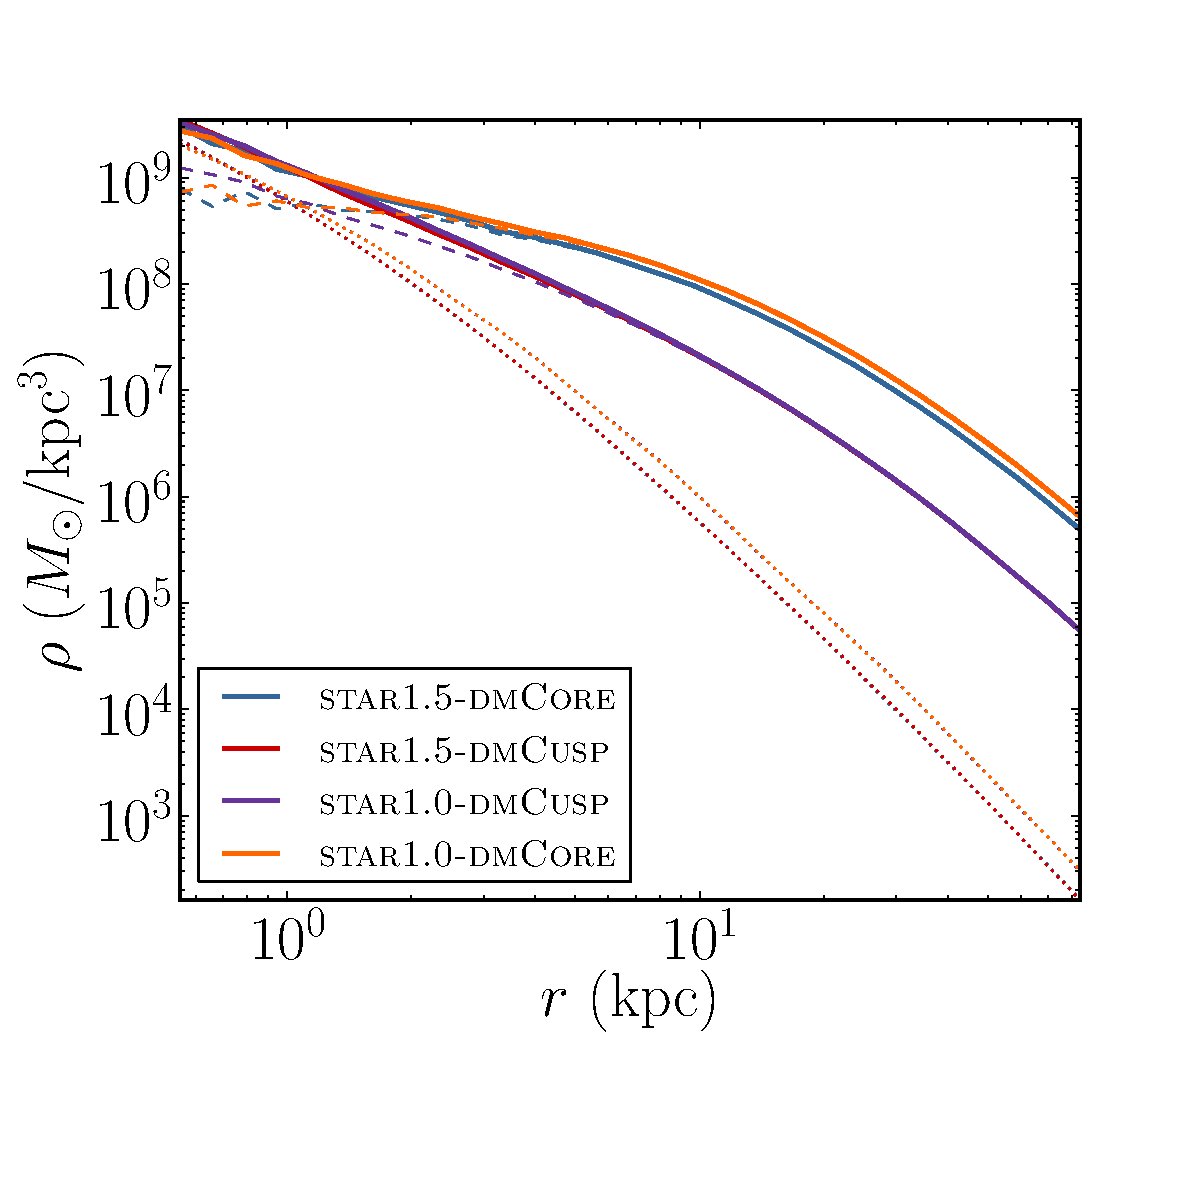
\includegraphics[width=0.33\textwidth]{MockGalProfile-a.pdf} 
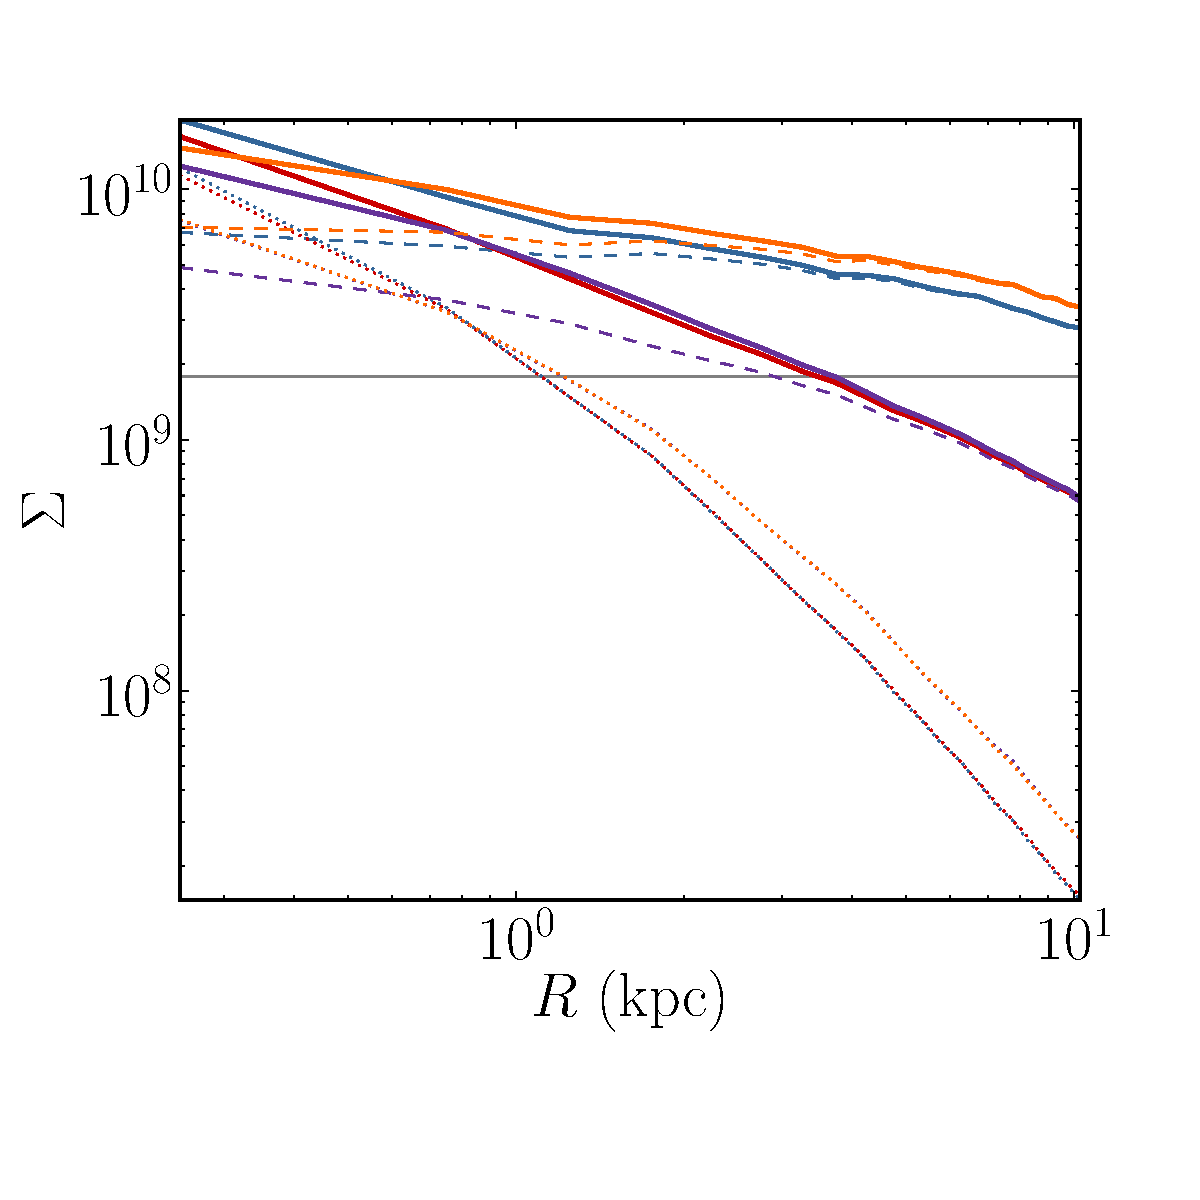
\includegraphics[width=0.33\textwidth]{MockGalProfile-b.pdf} 
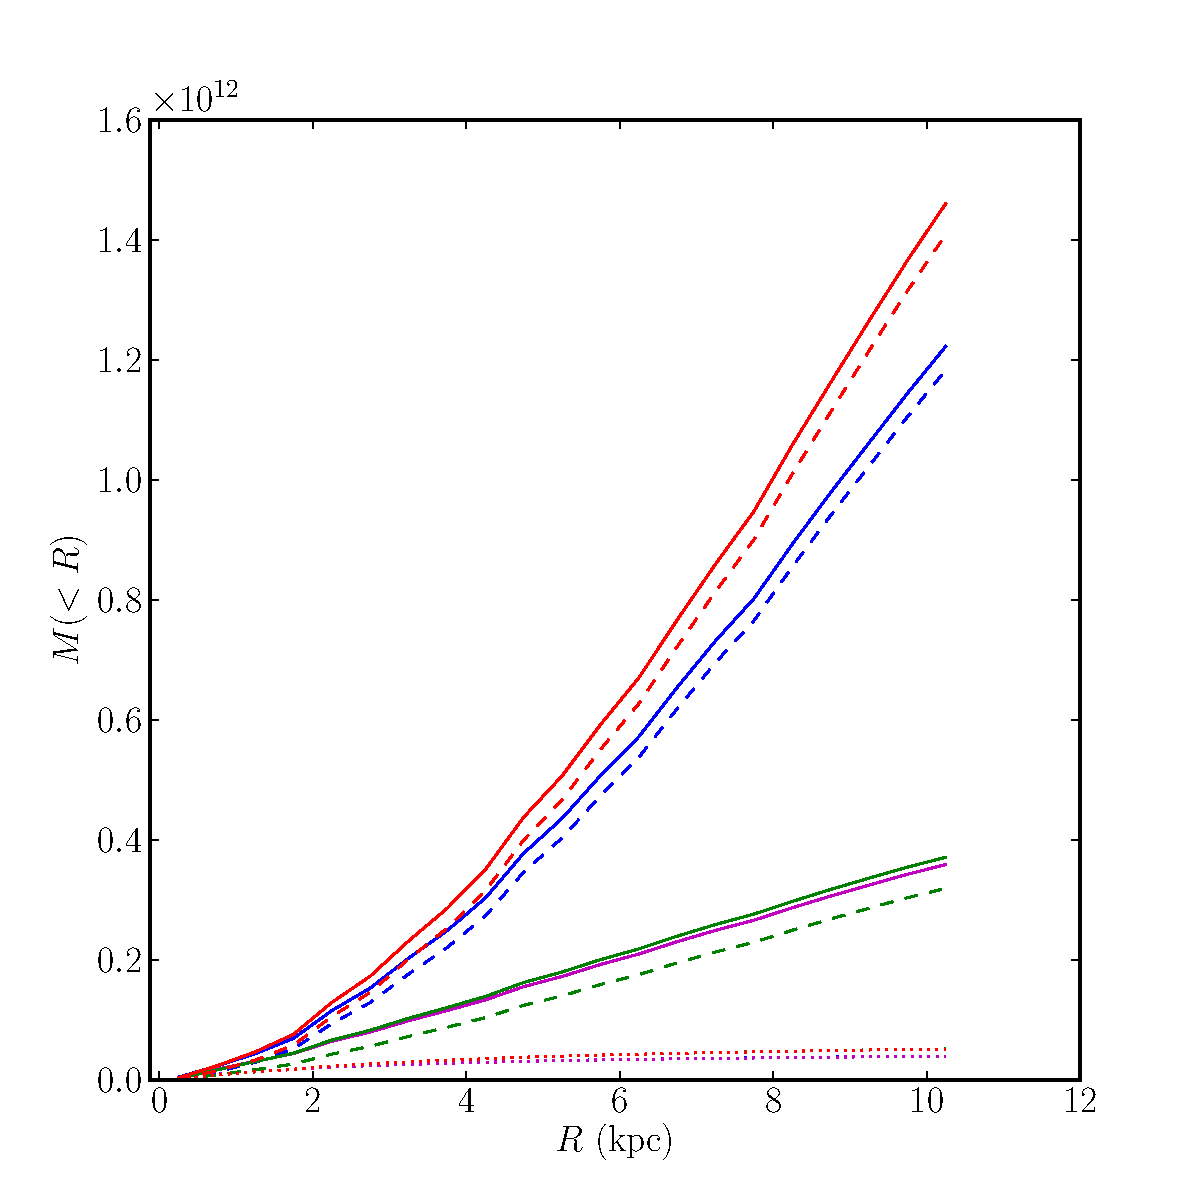
\includegraphics[width=0.33\textwidth]{MockGalProfile-c.pdf}
\caption{{\bf JR. \sout{Cut the analytic profiles from this Figure. All fonts and labels should be larger.} Left panel should start at 0.7kpc.}
\textbf{Left:} 
Spherically averaged density profiles of the four mock galaxies showing the stellar (dotted), dark matter (dashed),
and total (solid) densities. Notice that the stars in models Sdom/DMshallow and Sdom/DMcuspy contribute significantly to the central potential. 
\textbf{Middle:} 
The radially averaged two-dimensional projected density.
The critical density for lensing at $z_L=0.31$, $\kappa_\mathrm{crit}\sim 1.8\e{9}$\Msun/kpc$^2$, is marked by the horizontal line. 
\textbf{Right:}
The enclosed projected mass.
}
\label{mock galaxies}
\end{figure*}

In \figref{mock galaxies}, we show the 3D radial density, 
the 2D projected density, and the 2D enclosed mass for each
galaxy.

\subsection{Lens configurations}\label{sec:lensconfig} %--------------------------------------------------------------

For each of the four galaxies, we used the raytracing feature of \Glass\
described in \secref{Raytracing} to construct 6 basic lensing morphologies:

\begin{enumerate}
\item one double and one extended double;
\item one quad and one extended quad;
\item two 2-source quads with varying redshift contrast.
\end{enumerate}
The `extended' configurations use multiple point sources at the same redshift
to simulate an extended source that will produces an arc-like image.
\figref{arrival surfaces} shows the configuration for the extended quad, along
with the other cases. 

\begin{figure*}
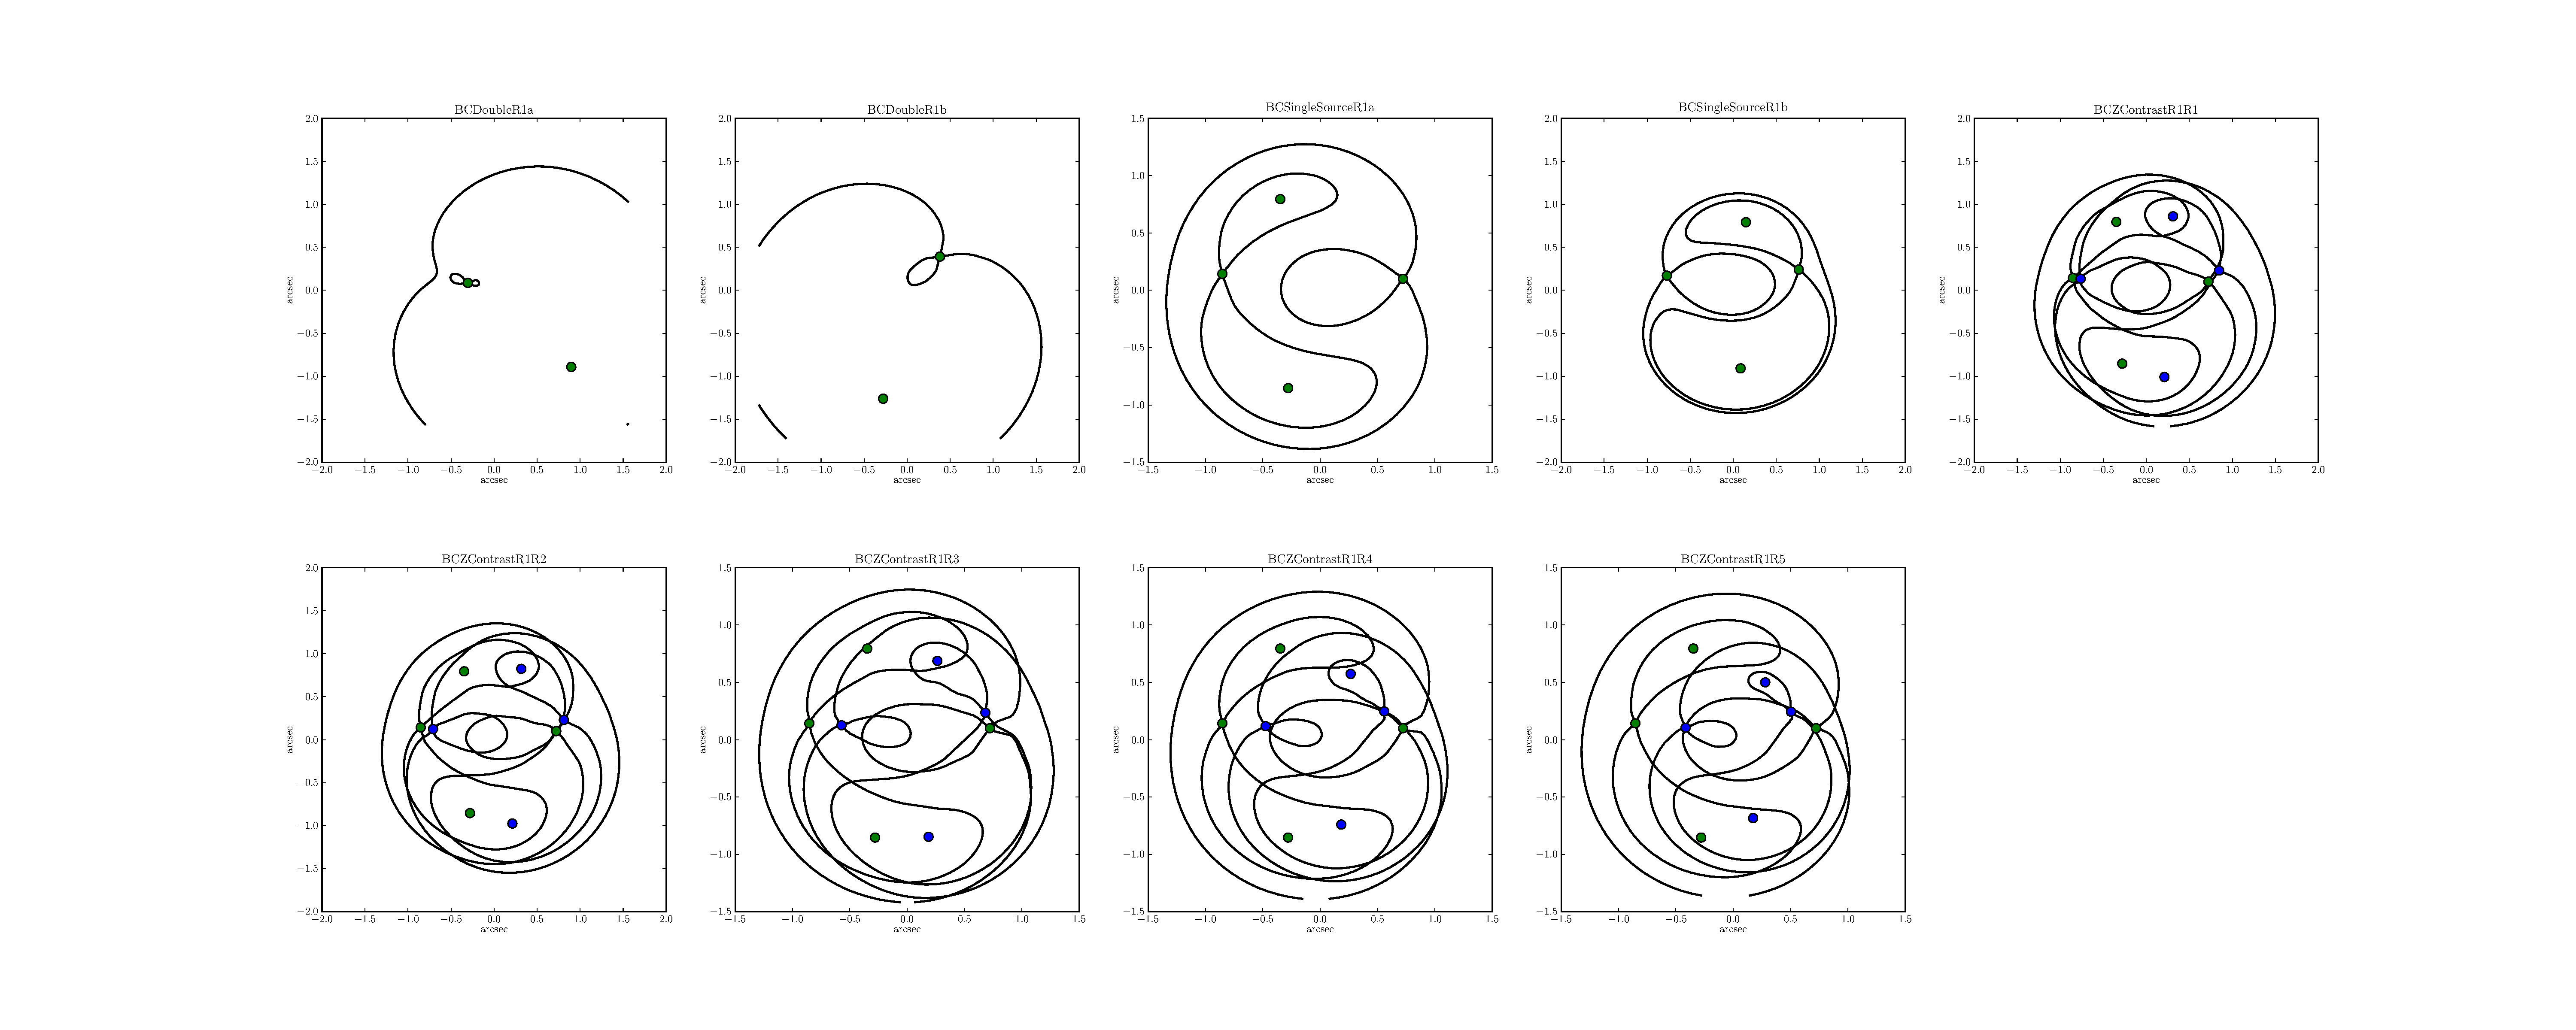
\includegraphics[width=0.85\textwidth]{BCarrival_surfaces}
\caption{The lens configurations for the six test cases using the BC mock galaxy. Here,
the central image is shown, although not all tests include it. The central image belongs
to only one set of images to avoid overconstraining the models. Similar colors group
images that share a common source. In the case of the extended image systems the source
is at the same redshift, while the redshift is varied between the systems in the 
ZConstrast cases. Grey circles are a visual aid to help determine radial separation
between images. The axes are measure in arcseconds.}
\label{arrival surfaces}
\end{figure*}

Each of these configurations were modelled with and without time delays and
with and without a central image, for a total of 24 test cases. (The central
image is typically highly demagnified. For galaxy lenses it is very difficult
to find since it lies along the sight line to the bright lensing galaxy; in
clusters, however, such images have been seen (CITES)). We assumed for all our
tests that the lensing mass was radially symmetric (Prior vi):
For our mock data, this is known to be
true; it is most often the case with real galaxies, unless there is an obvious
observed asymmetry. The central pixel was refined into a further 25 pixels to
capture any steep rise in the profile.  Two of the four mock galaxies have a
steeply rising inner profile. {\bf JR.  What happens if we don't assume this
symmetry? We ought to add an appendix showing this for one example case.}

\section{Results}\label{sec:results}
\figref{reconstruction} shows a typical reconstruction of a lens. The far left
plot shows the ensemble average arrival time surface with image marked as
circles and the inferred source position as a diamond. The center plot shows
the radial density profile. The error bars cover a $1\sigma$ range around the
median. \sout{the full range of models generated by \Glass {\bf JR. Why do
this? Surely 1 or 2 sigma errors make more sense? I've deleted the ``full
ensemble'' results and kept the $1\sigma$ ones instead.}}. The true density
profile from the mock data is also plotted for comparison. The vertical lines
mark the radial position of the images. The final plot on the right is of the
enclosed mass. As expected, the error bars are smallest in the region of the
images where the most information about the lens is present. The dip in the
profile at the end of the profile is due to the cut off in mass in the
lensing map. This is of little importance, though, as there is no lensing
information there.

\begin{figure*}
  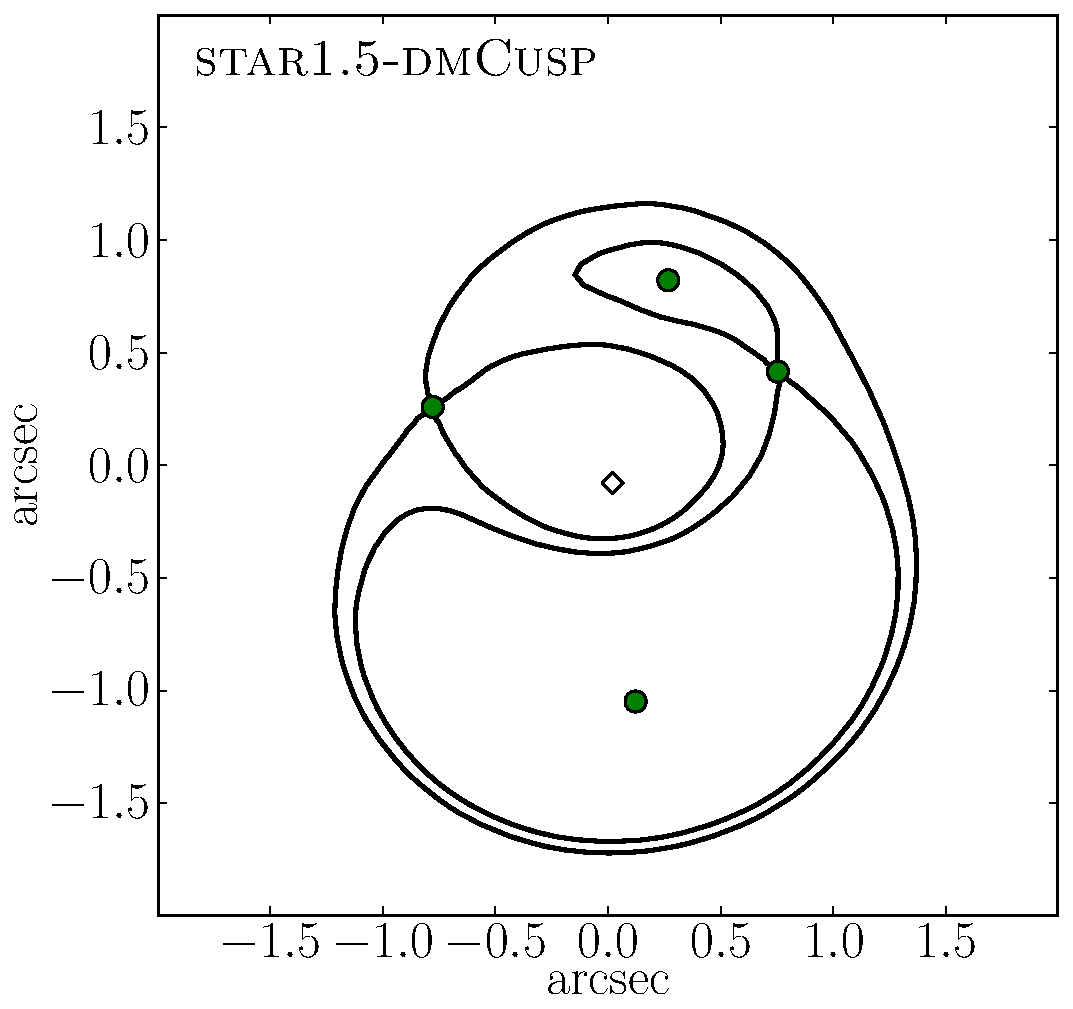
\includegraphics[width=0.35\textwidth]{BCQuadR1a_TmS-a.pdf}\hspace{-2em}
  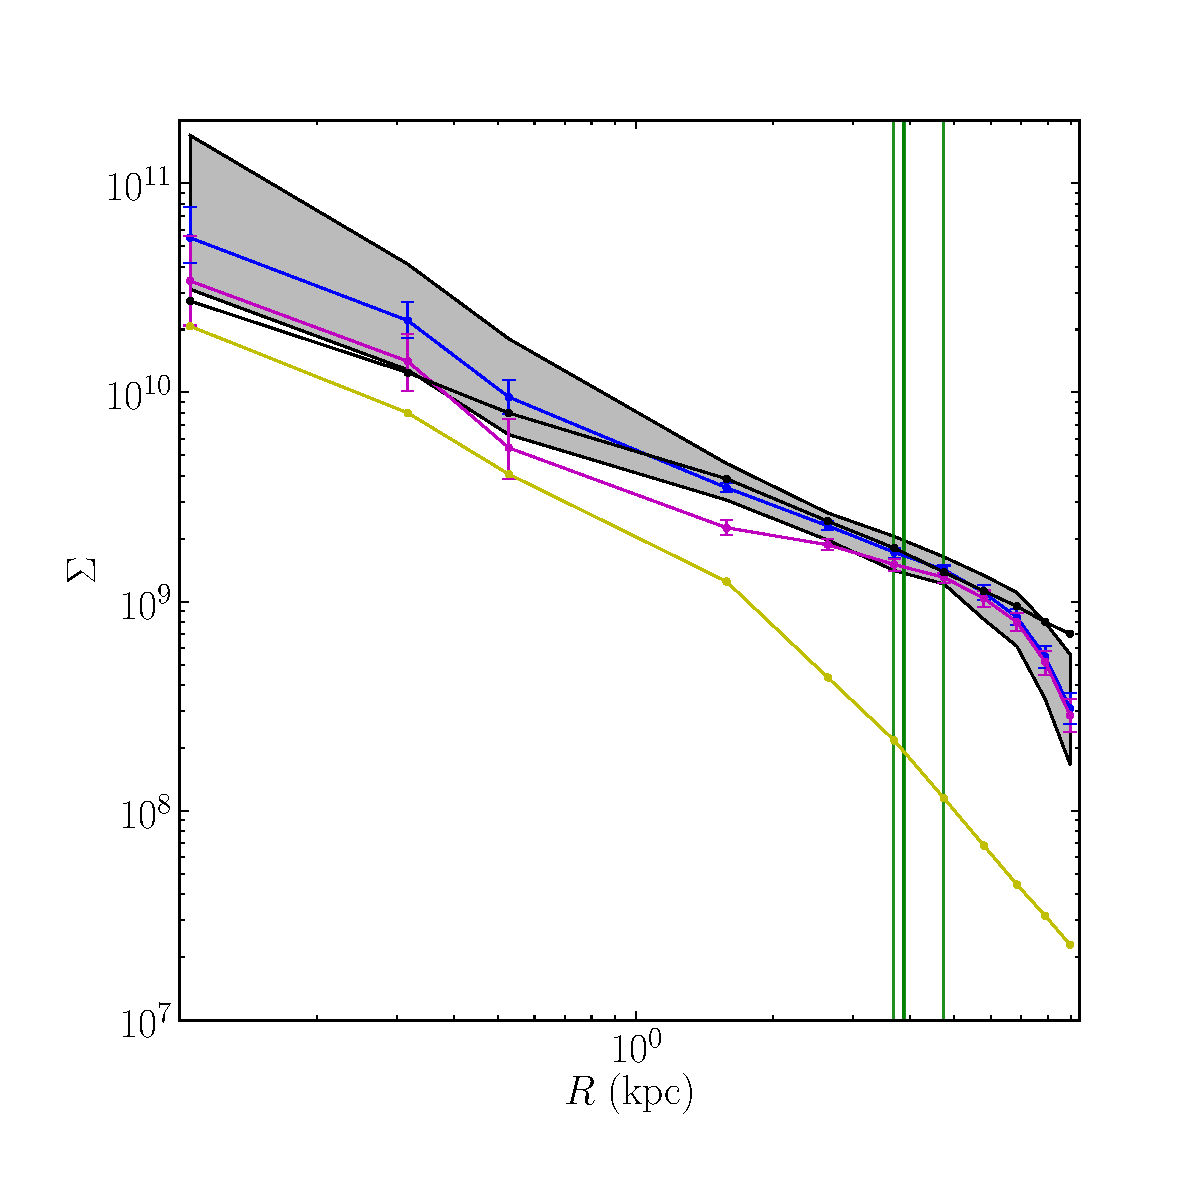
\includegraphics[width=0.35\textwidth]{BCQuadR1a_TmS-b.pdf}\hspace{-2em}
  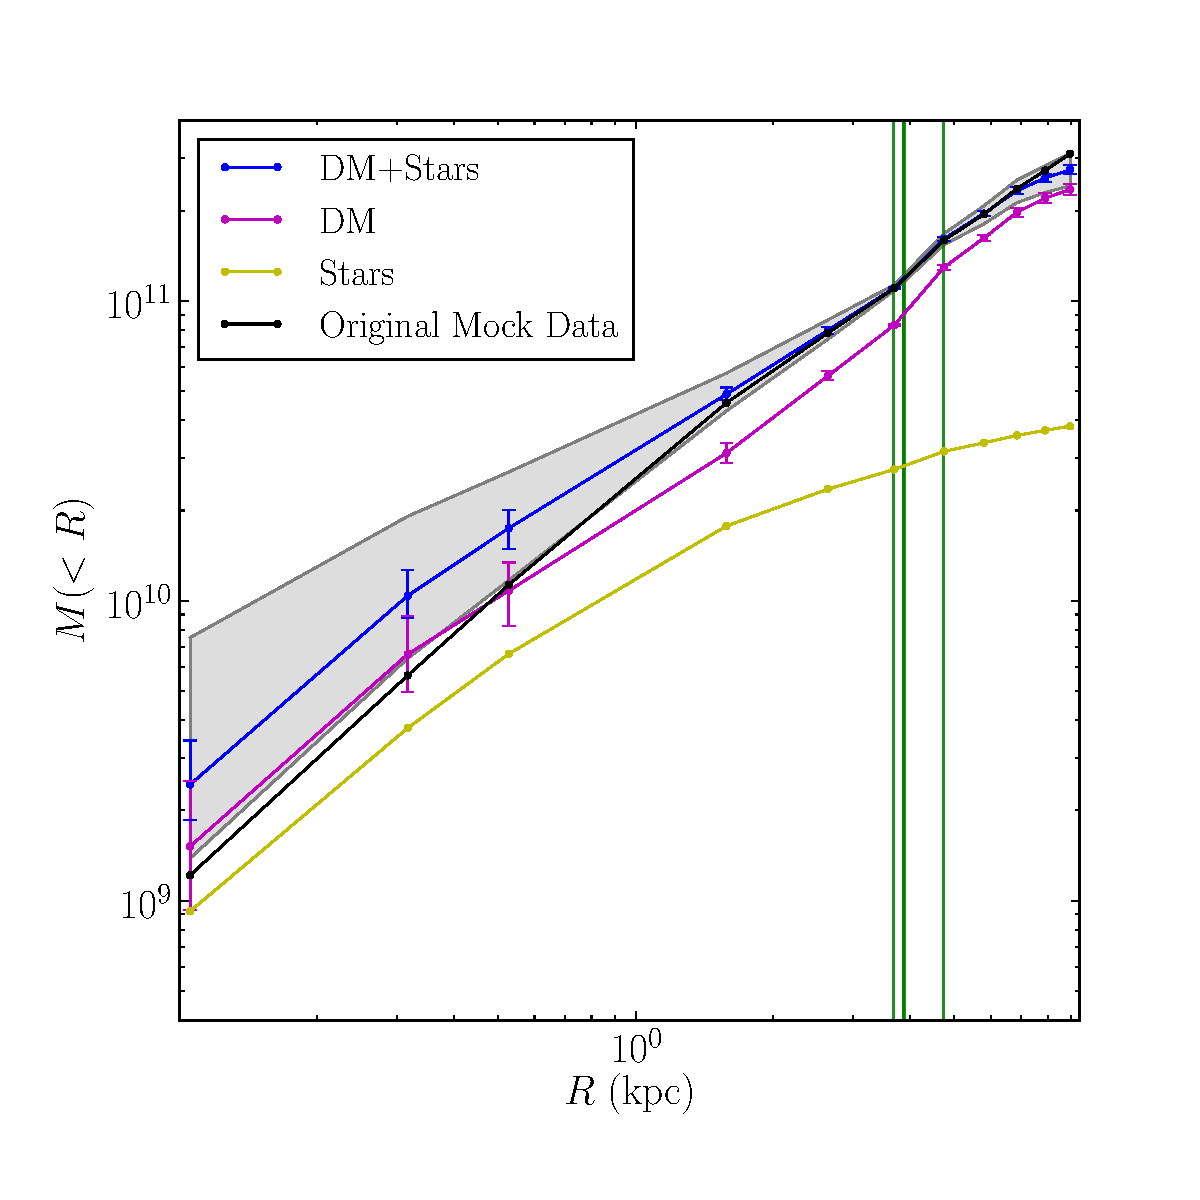
\includegraphics[width=0.35\textwidth]{BCQuadR1a_TmS-c.pdf}\\\vspace{-1em}
  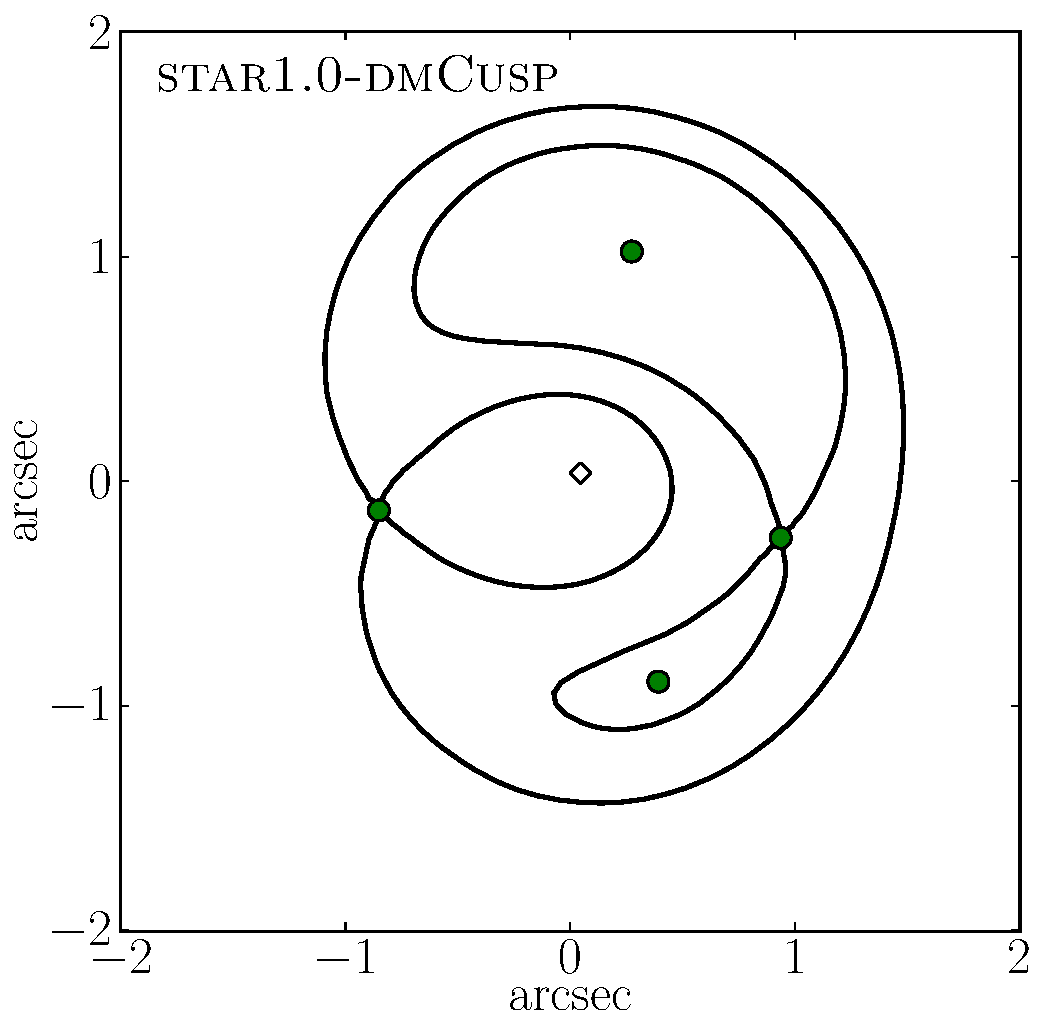
\includegraphics[width=0.35\textwidth]{ACQuadR1a_TmS-a.pdf}\hspace{-2em}
  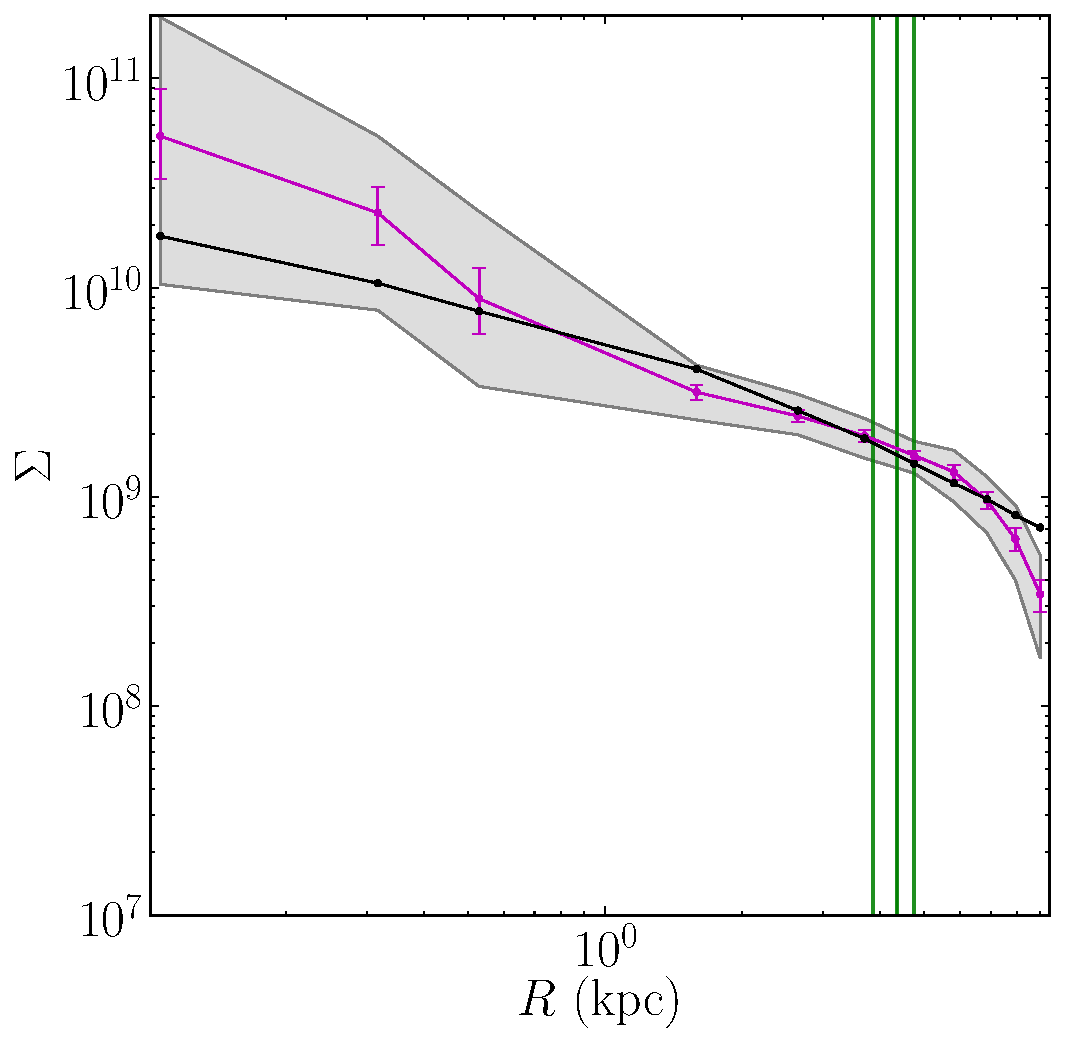
\includegraphics[width=0.35\textwidth]{ACQuadR1a_TmS-b.pdf}\hspace{-2em}
  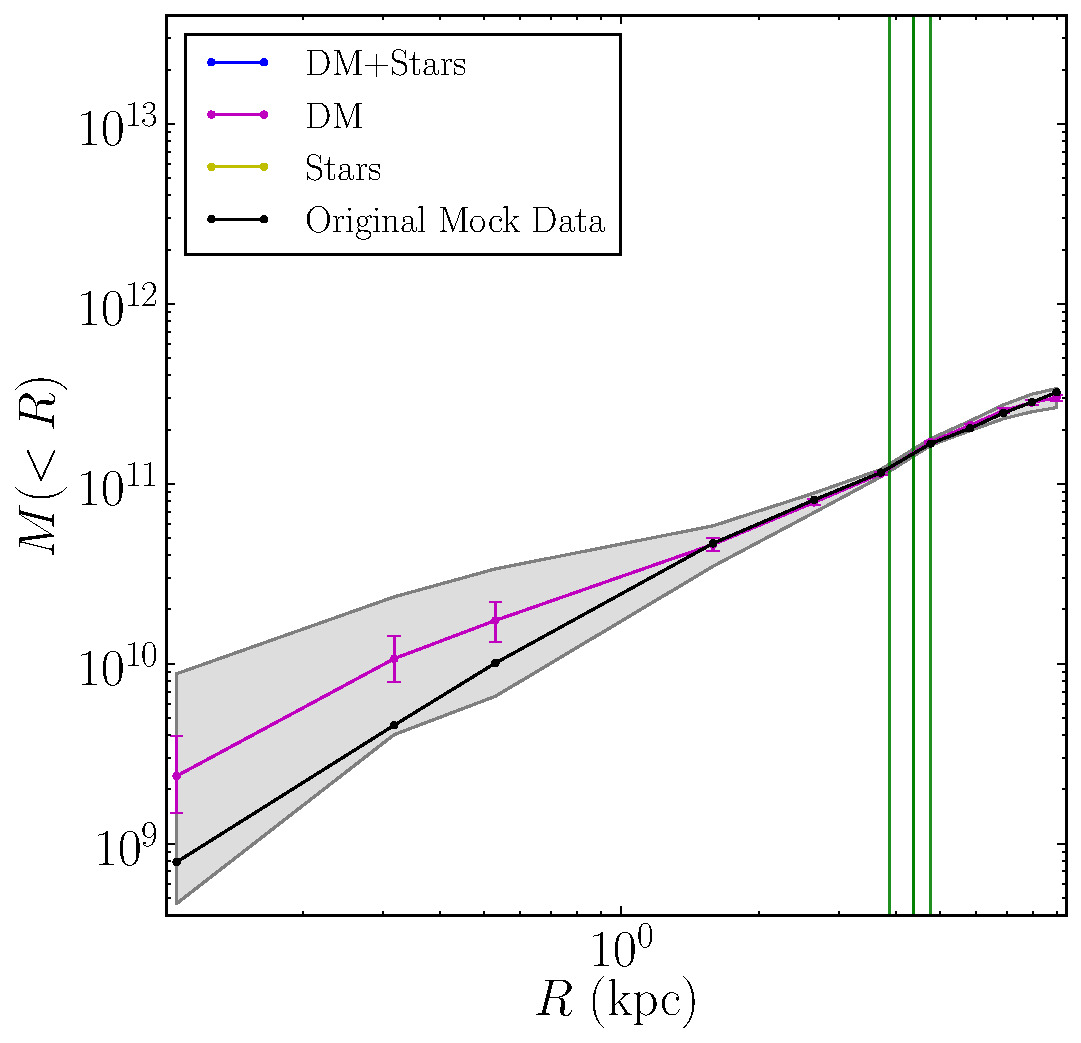
\includegraphics[width=0.35\textwidth]{ACQuadR1a_TmS-c.pdf}
\caption{
  \sout{{\bf JR. Need to homogenise plot dimensions here. Larger fonts as in Figure 1 are also required.} }
A typical reconstructed lens. Here we present results for a single quad image lensed by the Sdom/DMcuspy mock galaxy.
\textbf{Left:}
The arrival time surface. 
\textbf{Middle:}
The surface density. The magenta curve represents the dark matter component,
the yellow curve the stellar component, and the blue curve is the sum of the two.
The black curve comes from the original mass model used to create the lens.
The green vertical lines mark the radial positions of the images. The higher
resolution feature of \Glass\ has been used on the central pixel allowing the
steep profile to be captured.
\textbf{Right:}
The cumulative mass. The error bars on all plots are $1\sigma$, but the grey area shows the full range for DM+Stars (blue).}
\label{reconstruction}
\end{figure*}

\begin{figure*}
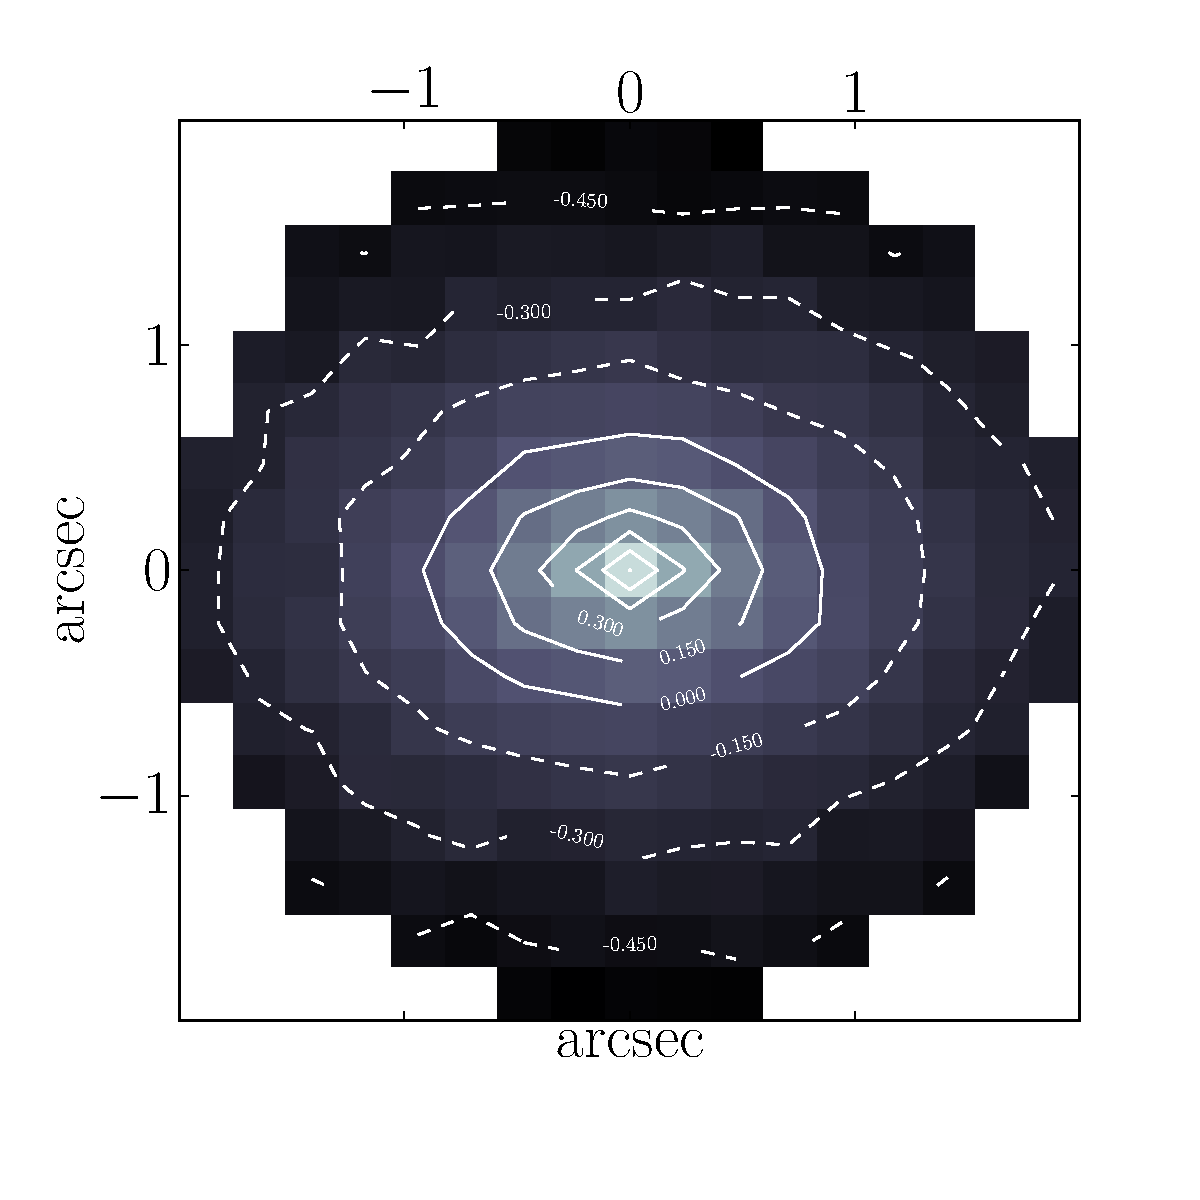
\includegraphics[width=0.33\textwidth]{BCQuadR1a_TmS-kappa-a.pdf}
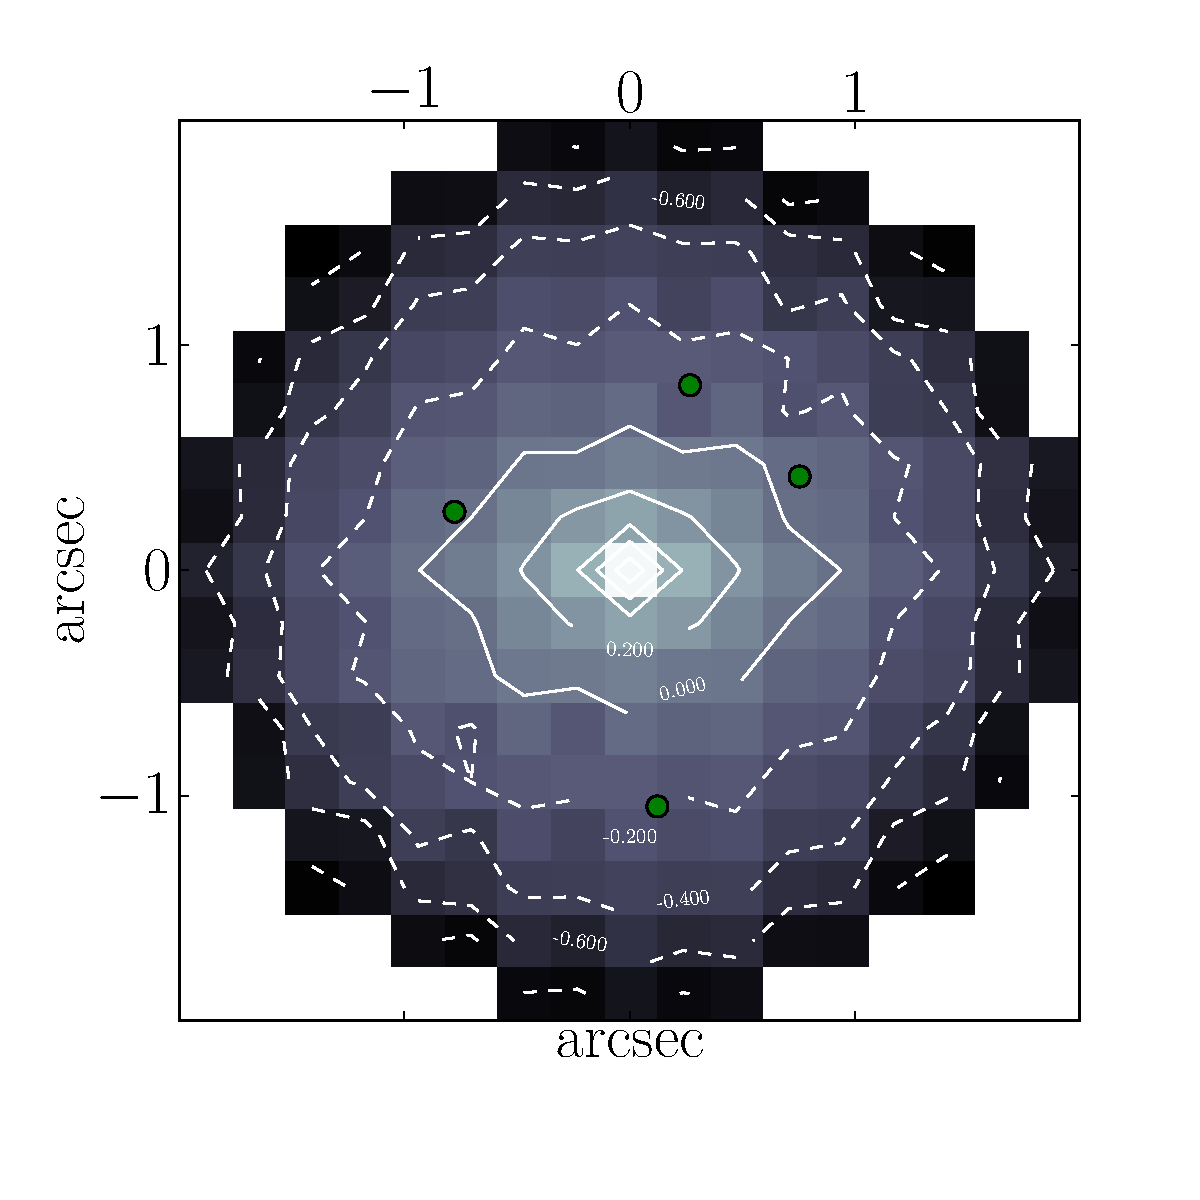
\includegraphics[width=0.33\textwidth]{BCQuadR1a_TmS-kappa-b.pdf}
\caption{ The mock data distribution for Sdom/DMcuspy on a coarse grid (left)
  and a typical recovered ensemble average $\kappa$ distribution. The contours are
  logarithmic values, where level 0 corresponds to the critical density.}
\label{2d mass reconstruction}
\end{figure*}

The main results from modeling these different configurations are shown in
\figref{main results} and \figref{main results pixel-wise}. Each
subplot corresponds to a different mock galaxy. We show the fractional error of the mass
distribution for each of the test configurations with (red) and without stellar mass (black)
In \figref{main results}, the error is defined over radial bins of mass as
%
\begin{equation} \label{badness}
  f_R = \frac {\sum_i \left|M_p(i) - \tilde M_p(i)\right| } {\sum \tilde M_p(i)}
\end{equation}
%
where $M_p$ is the mass in a radial bin and $\tilde M_p$ is the mass from the mock galaxy.
In \figref{main results pixel-wise} the error is defined over all the pixels $\vec\theta$
%
\begin{equation} \label{badness}
f_\theta = \frac {\sum_{\vec\theta} \left|M(\vec\theta) - \tilde M(\vec\theta)\right| } {\sum \tilde M(\vec\theta)}
\end{equation}
%
%\begin{equation}
%  \chi_i \equiv 100 \times \sqrt{\frac{\int_r (\rho_{\M_i}(r) - \rho_G(r))^2}{\int_r \rho_G(r)^2}}
%\chi_i = \frac{\sum_r (\rho(r)_{\M_i} - \rho(r)_G)^2}{\sum_r \rho(r)_G^2}
%\end{equation}
%where $\rho_{\M_i}(r)$ is the recovered density profile for a mock model $\M_i$; and $\rho_G(r)$ is the true density profile. 

\begin{figure*}
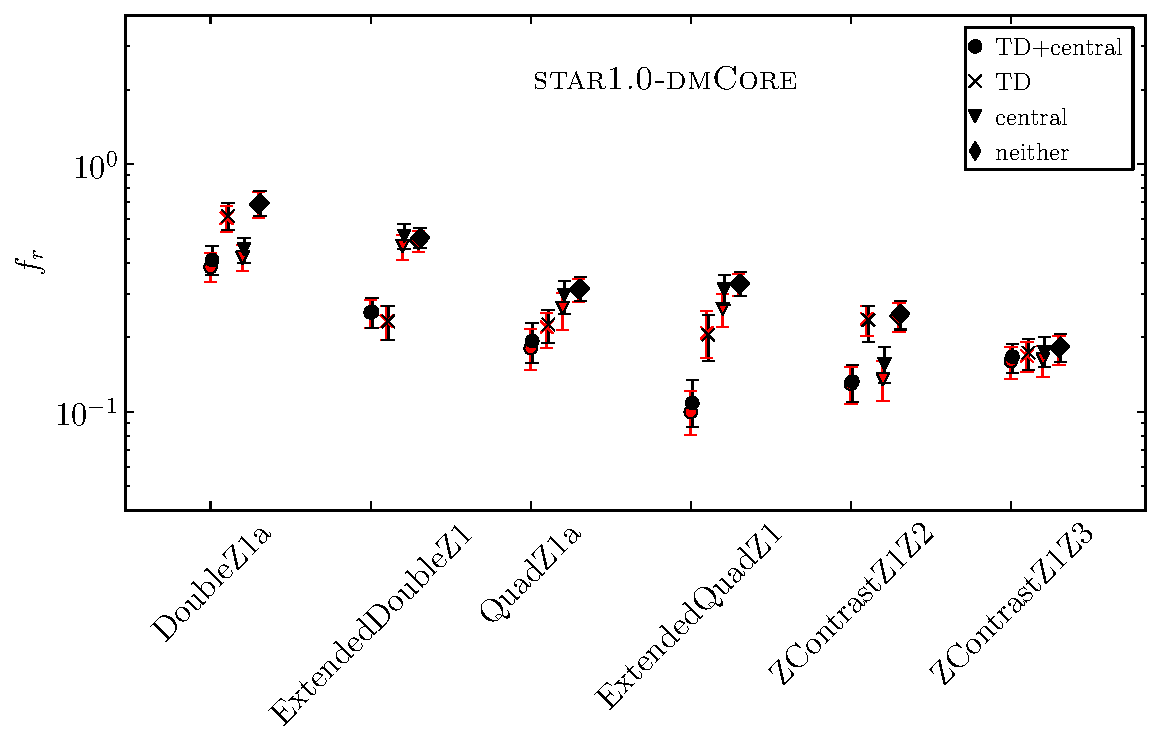
\includegraphics[width=0.49\textwidth]{AAferror_profile-1sig.pdf}
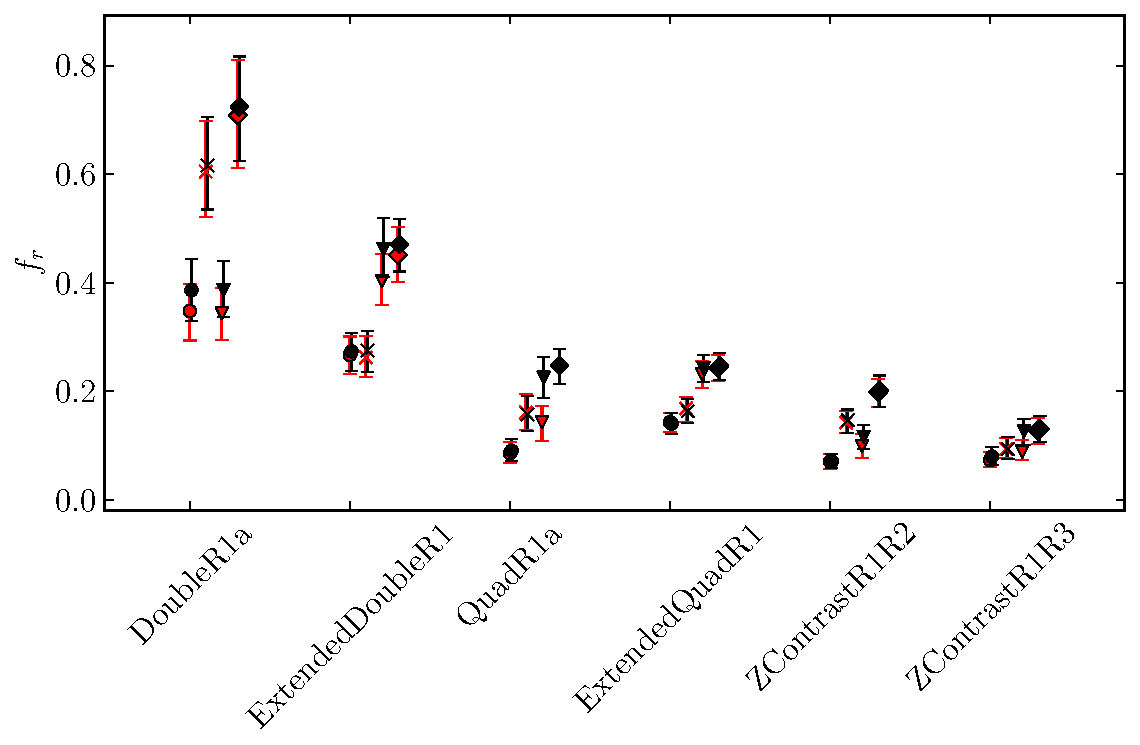
\includegraphics[width=0.49\textwidth]{BBferror_profile-1sig.pdf}\\
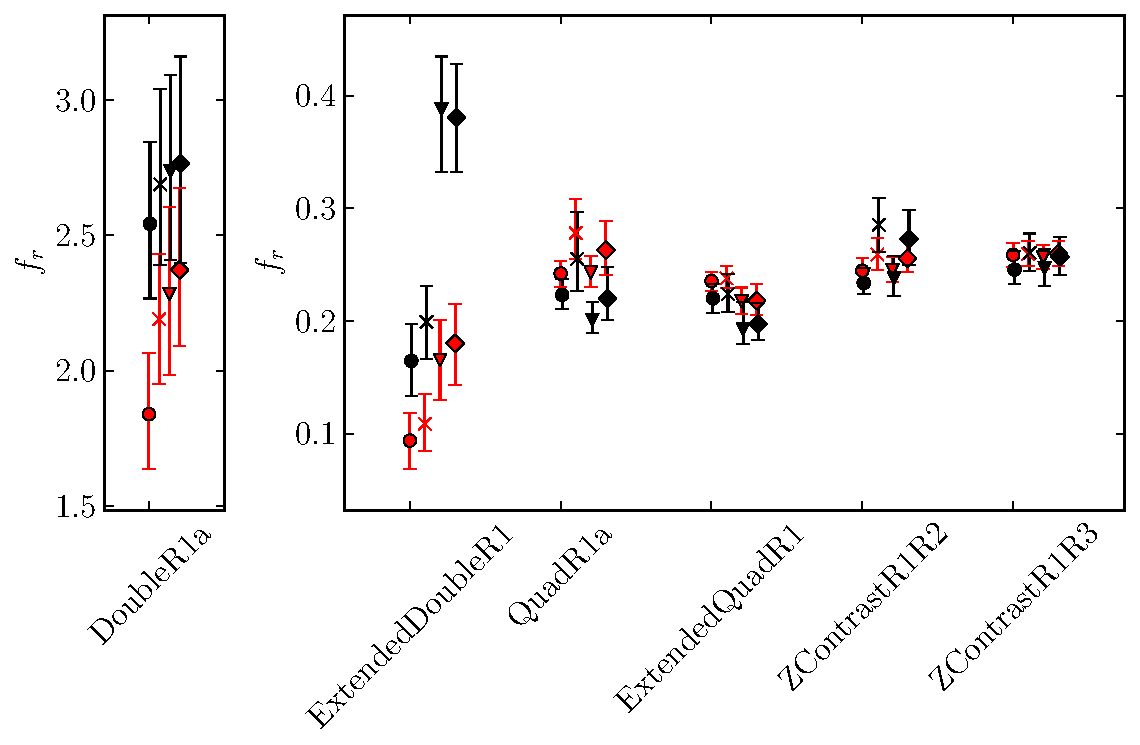
\includegraphics[width=0.49\textwidth]{ACferror_profile-1sig.pdf}
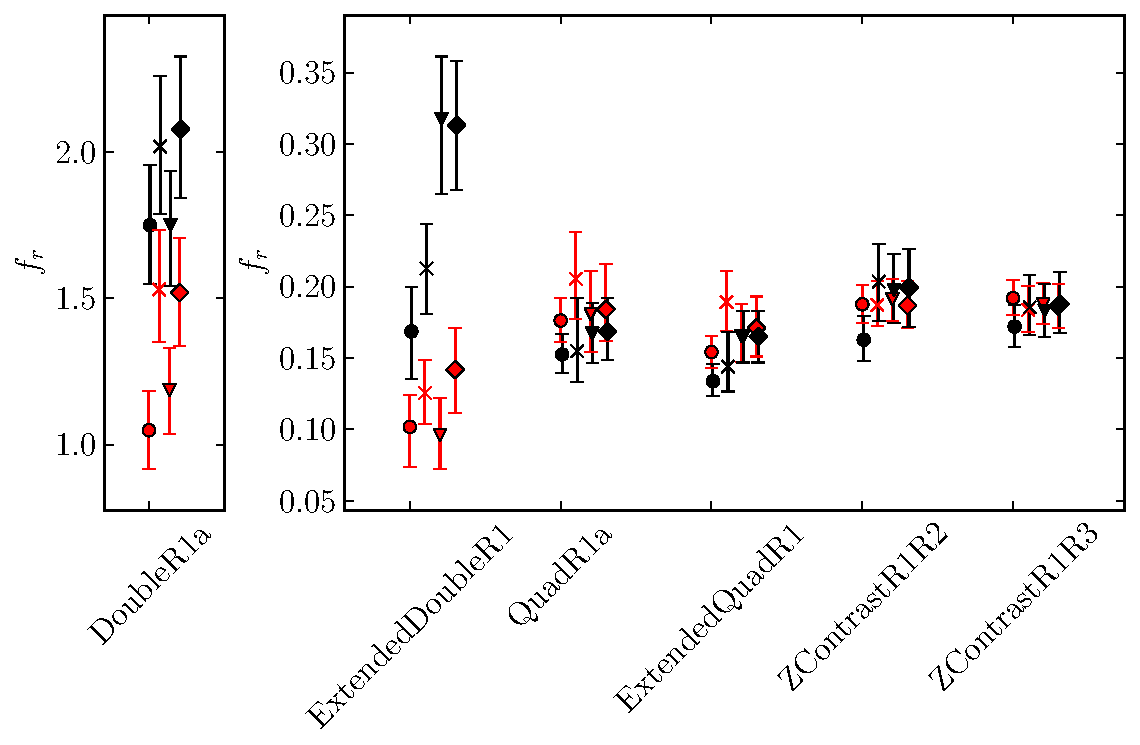
\includegraphics[width=0.49\textwidth]{BCferror_profile-1sig.pdf}
\caption{The main results showing the quality of model recovery. Each panel corresponds to 
the named mock galaxy, whose parameters are listed in \tabref{mock galaxy params}. Within
each panel are six groups of results for each of six lens morphologies. Each morphology
considered the presence of time delays (T/t) and a central image (M/m). The black markers are for tests
that did not include the stellar mass as a lower bound constraint, while the red markers
indicate where the stellar mass has been given. Error bars show the $1\sigma$ equivalent interval sampled from the model ensemble.}
\label{main results}
\end{figure*}

\begin{figure*}
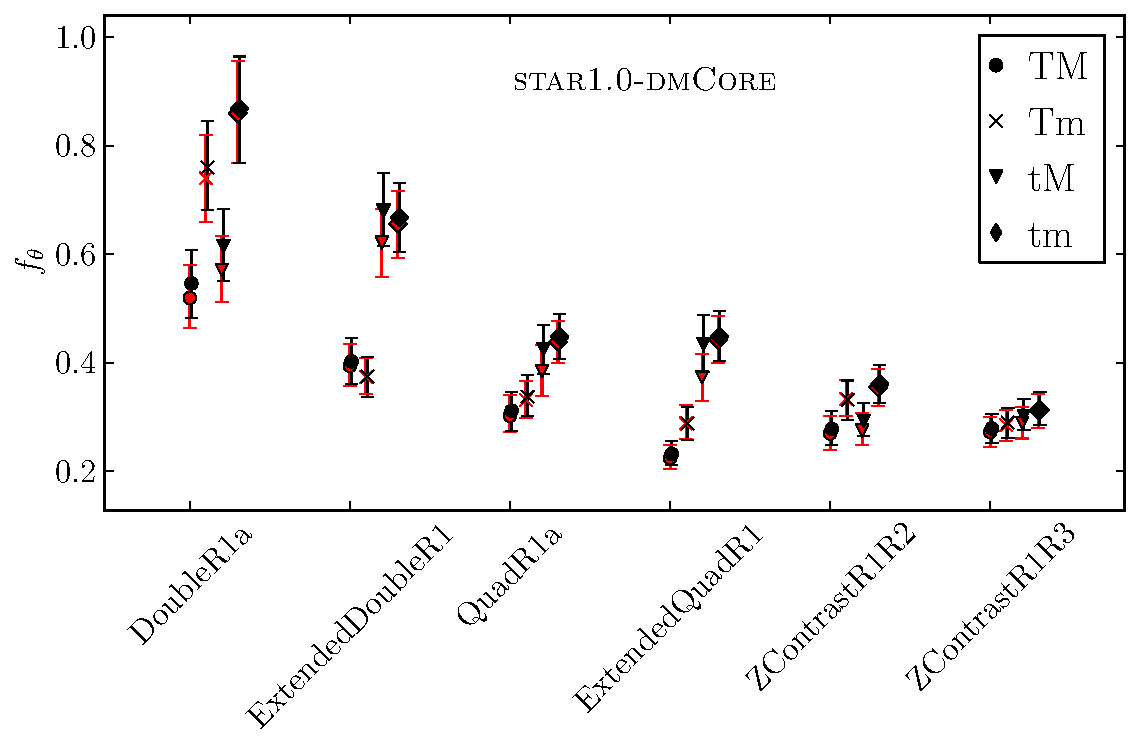
\includegraphics[width=0.49\textwidth]{AAferror-1sig.pdf}
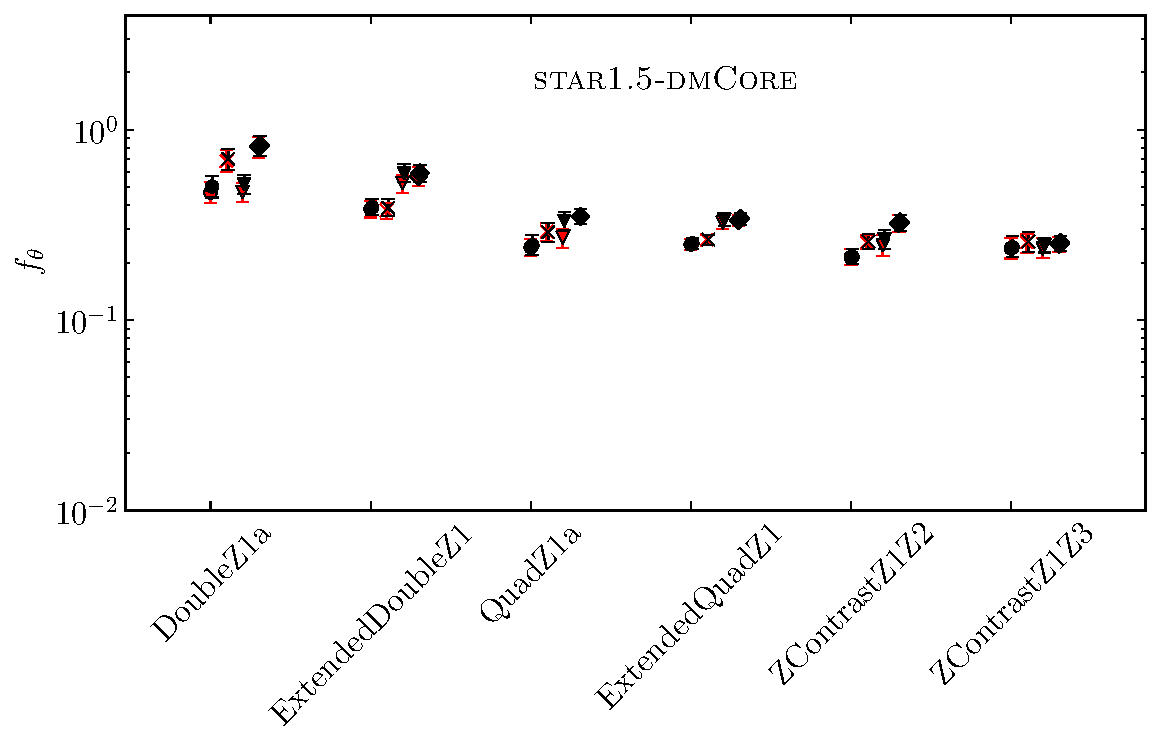
\includegraphics[width=0.49\textwidth]{BBferror-1sig.pdf}\\
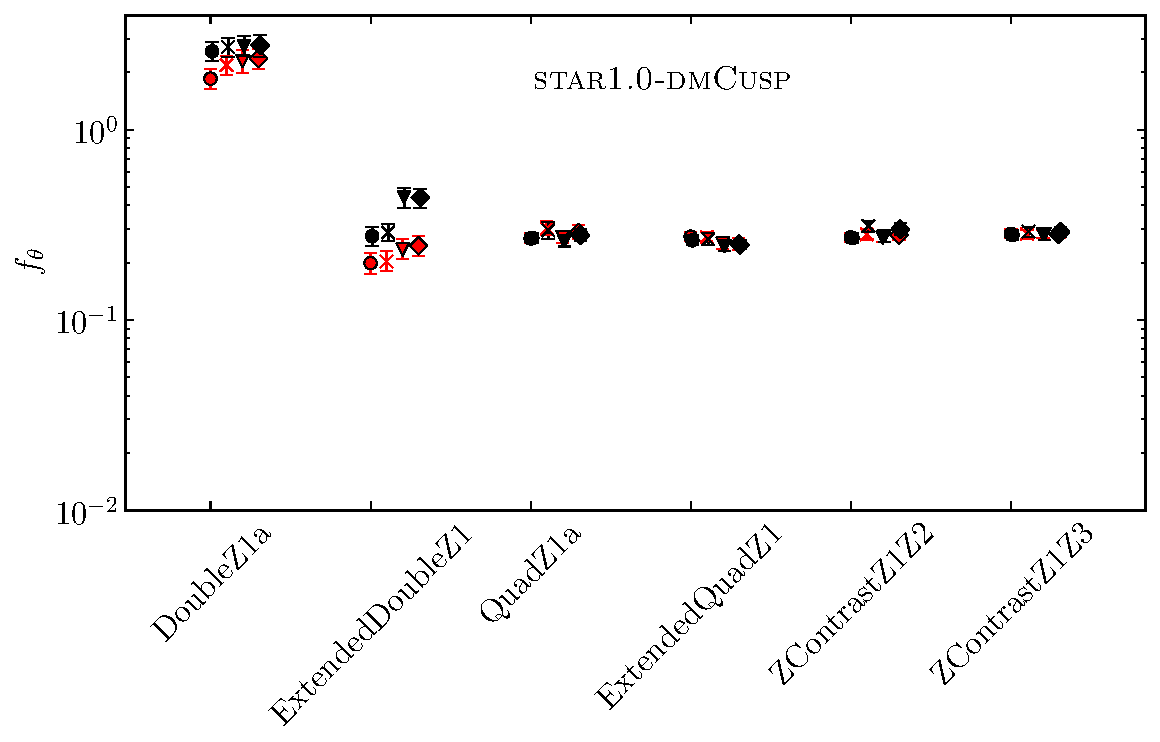
\includegraphics[width=0.49\textwidth]{ACferror-1sig.pdf}
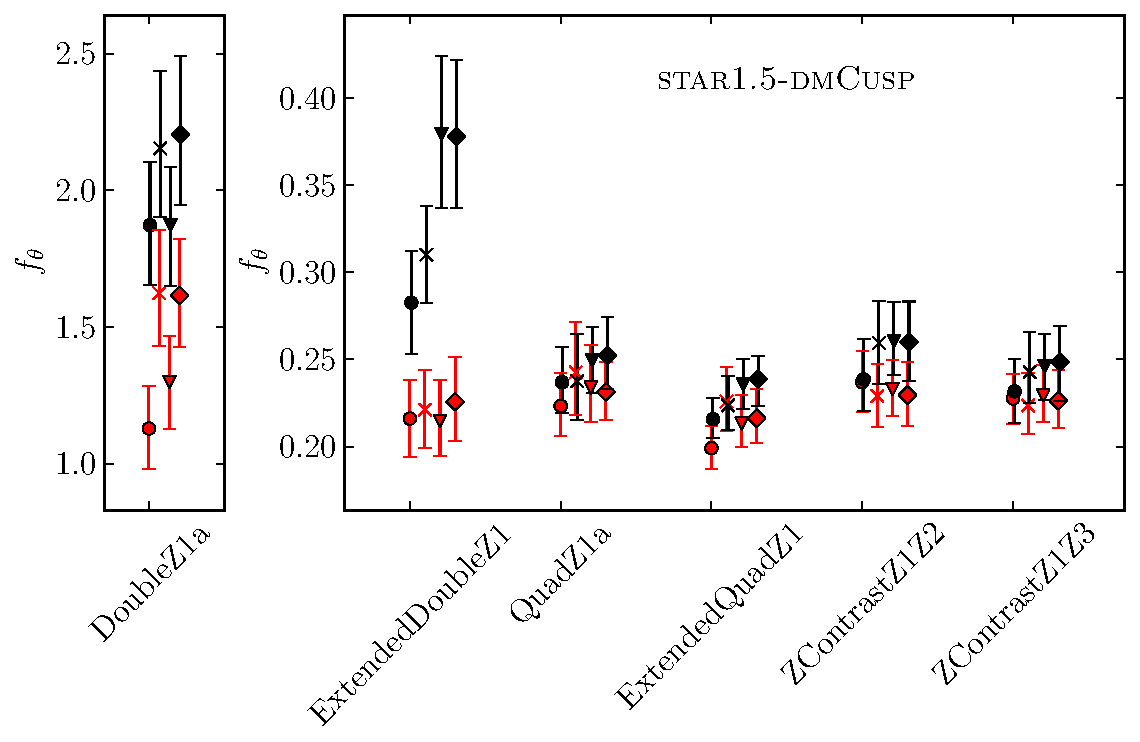
\includegraphics[width=0.49\textwidth]{BCferror-1sig.pdf}
\caption{ {\bf JR. \sout{ This should be also with $1\sigma$ errors.} Also need to do this plot for Claudio's shape measure.} \sout{Pixel-wise $\chi$.}
The fractional error for the pixel-wise recovery of all models. The colors and labels are the same as in \figref{main results}. Error bars show the $1\sigma$ equivalent interval sampled from the model ensemble.}
\label{main results pixel-wise}
\end{figure*}

\begin{figure}[h]
\plottwo{AAExtendedDoubleR1_TmS-shape-hist-11.pdf}{BCZContrastR1R3_TmS-shape-hist-212.pdf}
\caption{ The two plots in the left most column show sample distributions of
  $s=\lambda_1/\lambda_2$, the ratio of the largest to smallest principal axes.
  The upper (poor) plot is from the DMdom/DMshallow galaxy, while the lower (good) plot is
  from the Sdom/DMcuspy galaxy. The black vertical lines mark the $1\sigma$
  region and the vertical blue line is the value of $s$ for the corresponding
mock galaxy. }

\label{shape results}
\end{figure}

\begin{figure*}
  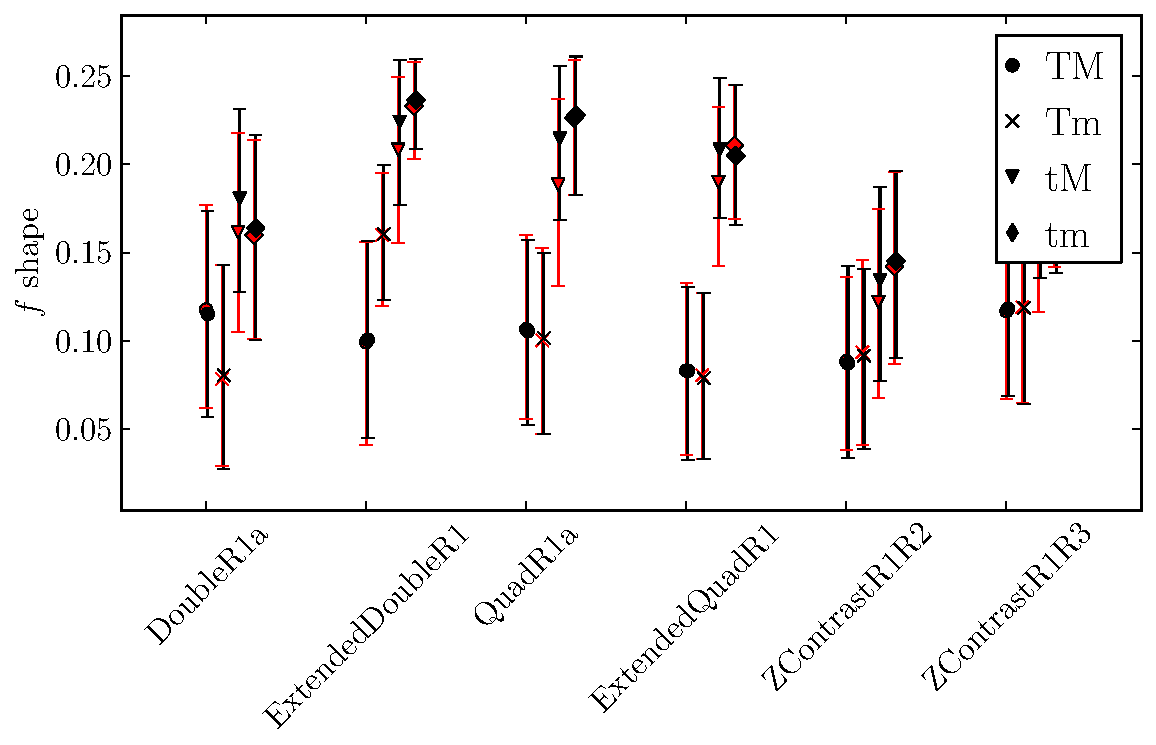
\includegraphics[width=0.33\textwidth]{AAferror_shape-1sig.pdf} \hspace{2cm}
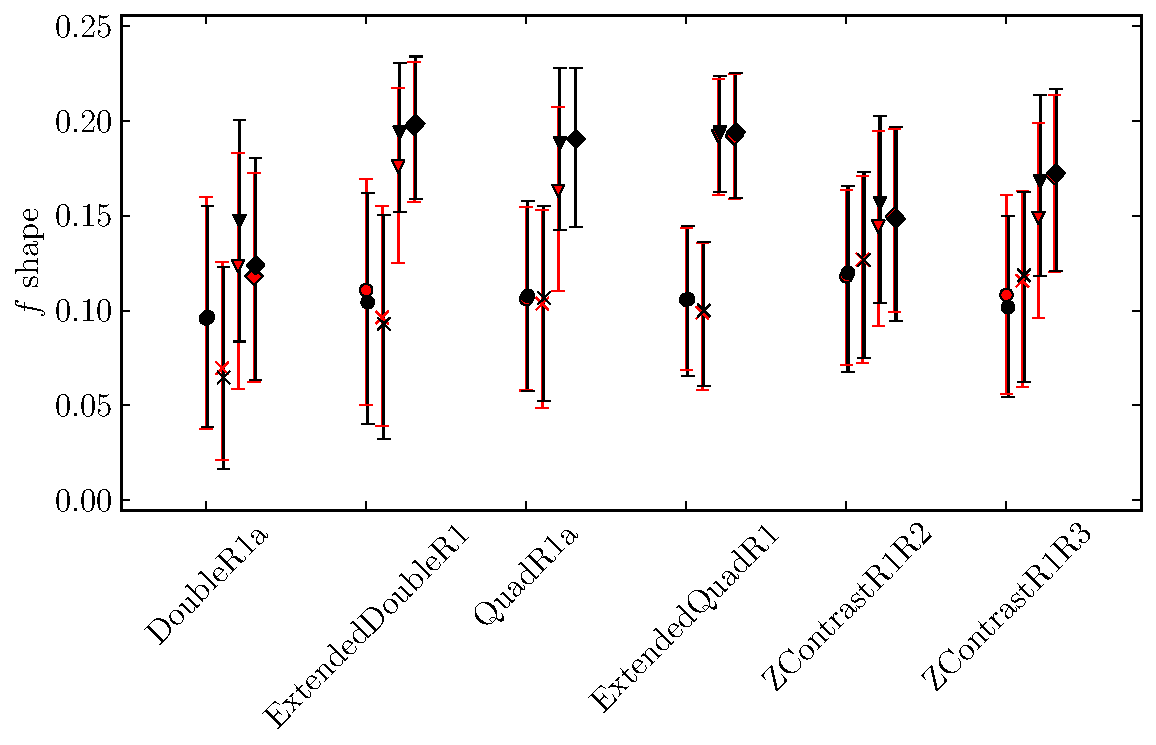
\includegraphics[width=0.33\textwidth]{BBferror_shape-1sig.pdf}\\
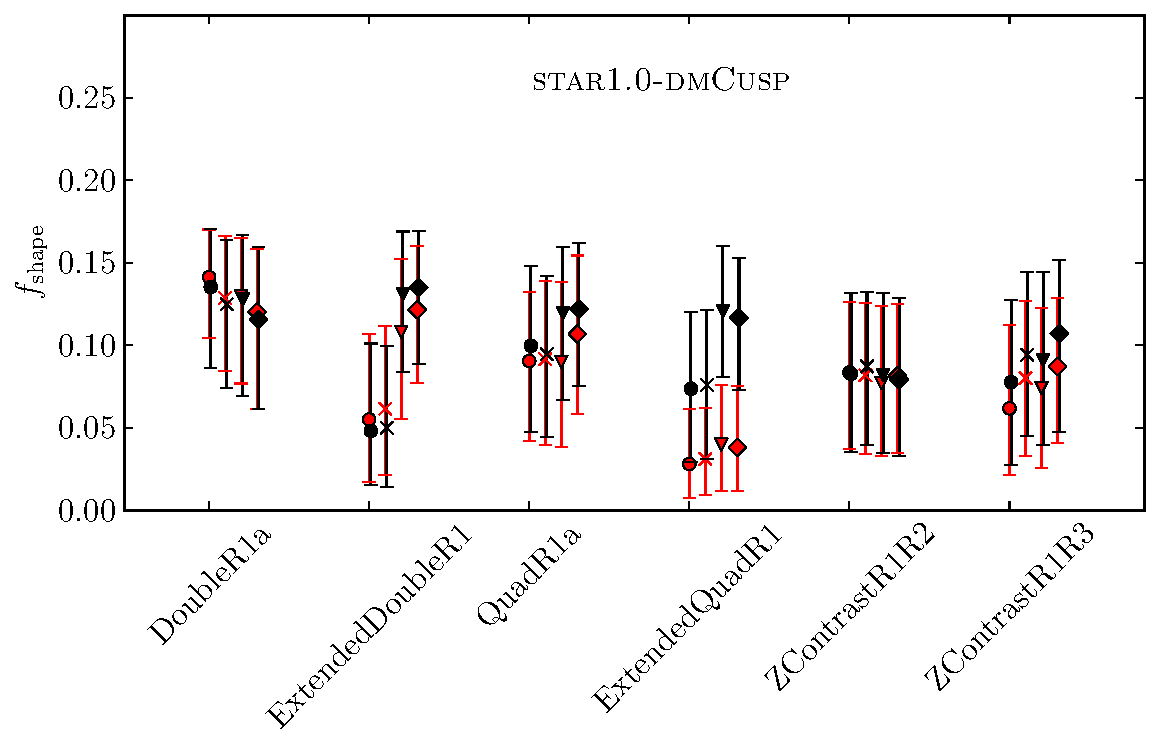
\includegraphics[width=0.33\textwidth]{ACferror_shape-1sig.pdf}\hspace{2cm}
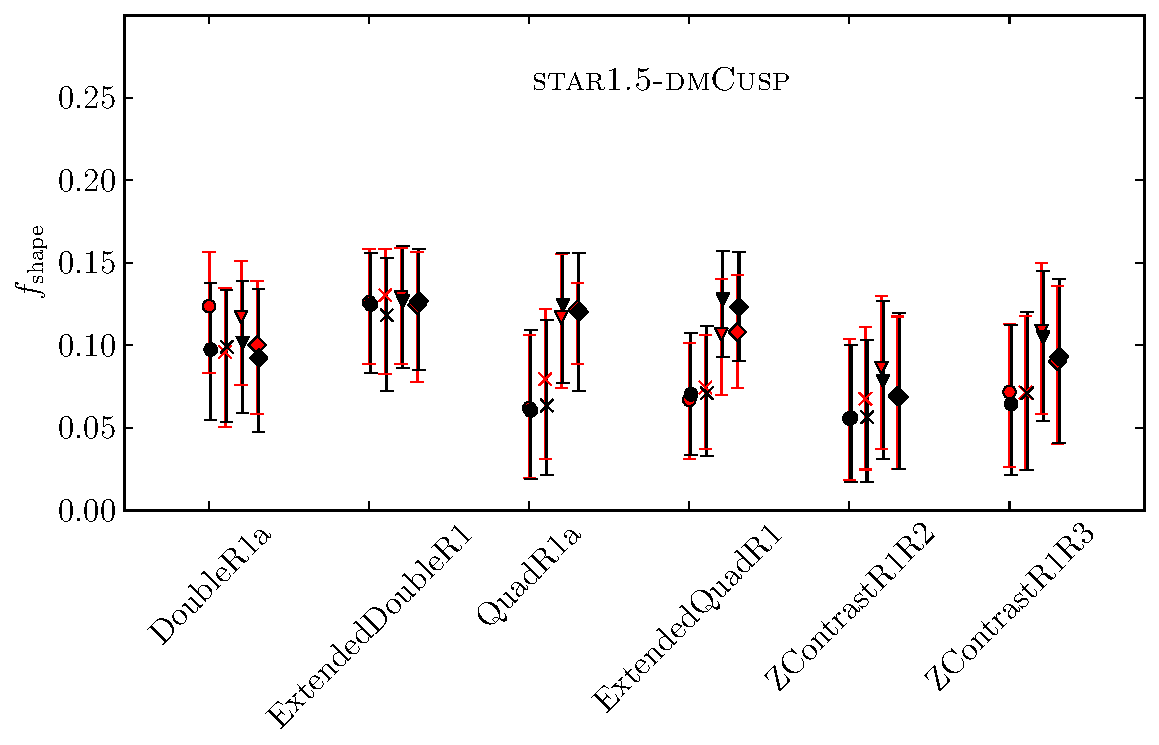
\includegraphics[width=0.33\textwidth]{BCferror_shape-1sig.pdf}
\caption{ The remain four plots are similar to those in \figref{main
  results pixel-wise} and show the fractional error of $s$ over all the models,
with respect to the mock galaxies.}

\label{shape results}
\end{figure*}

The abundance of strong lensing data increases from left to right within each plot. As
a result, there is a general trend for the reconstruction quality to increase
(and for $f$ to decrease). By adding more measurable information to each
configuration the quality can also be affected. When both time delays and a
central image are present the quality is highest. A double is known to provide
very little constraint on the mass distribution. This is particularly evident in
galaxies AC and BC where the mass profile is steepest and the reconstruction of
the double is poorest. However, the addition of an arc is sufficient to correct
this.

\begin{figure*}
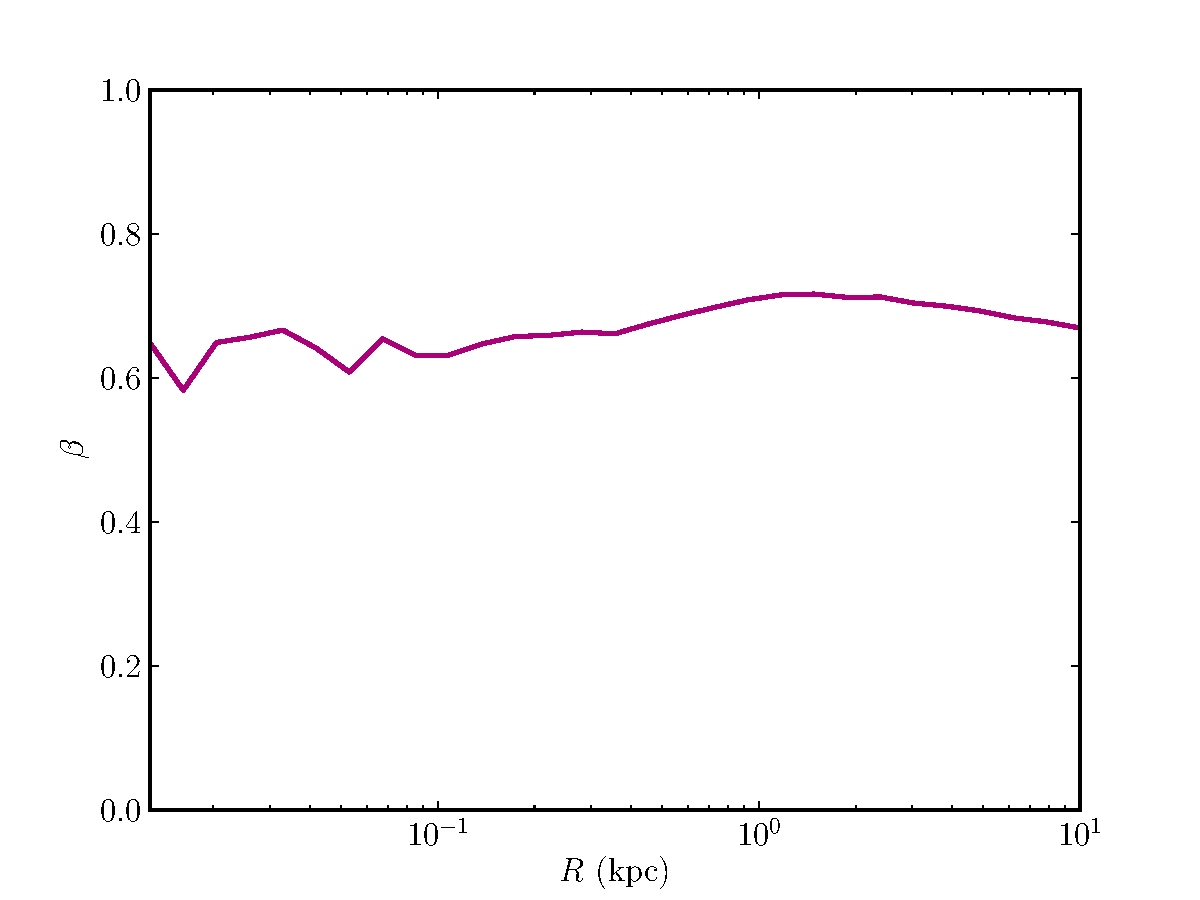
\includegraphics[width=0.33\textwidth]{BC_beta.pdf}
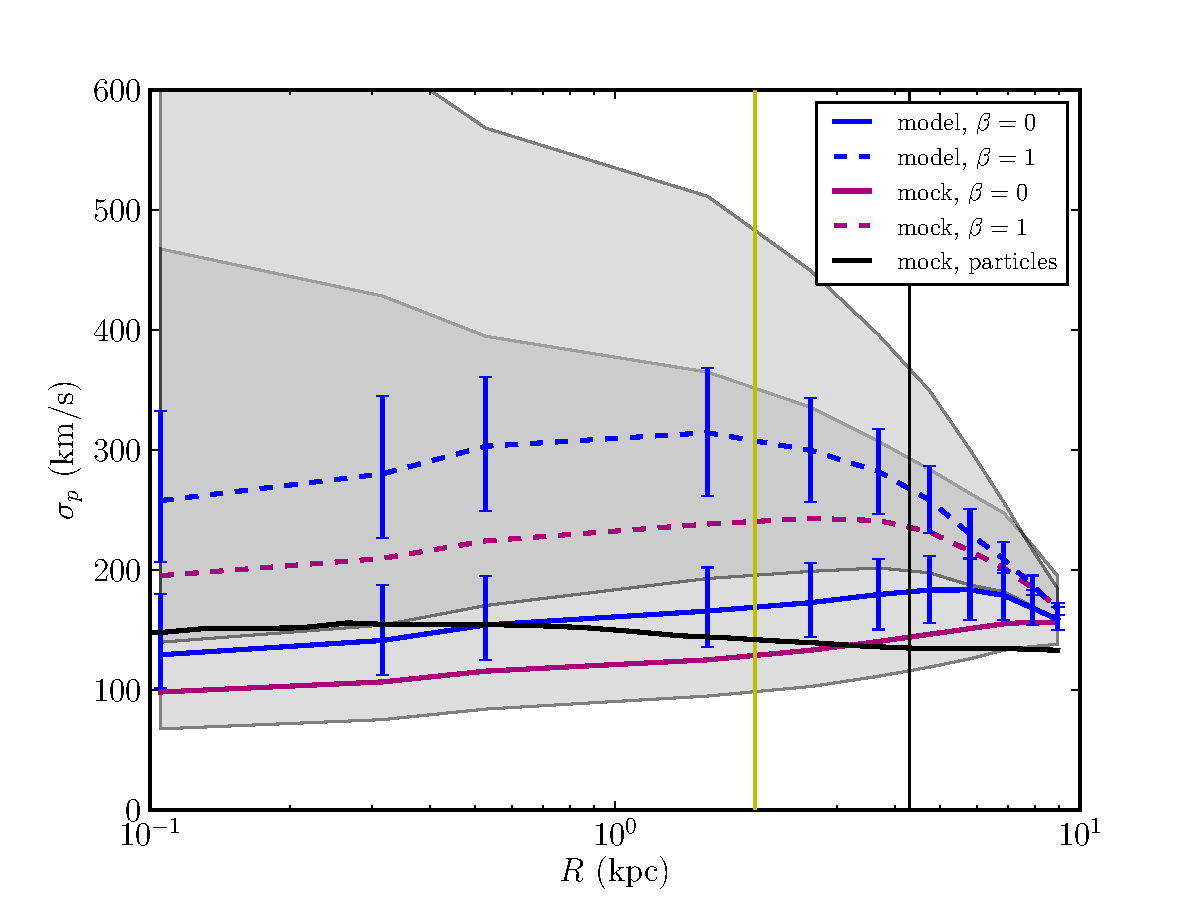
\includegraphics[width=0.33\textwidth]{BCQuadR1a_Tms_sigp-1.pdf}
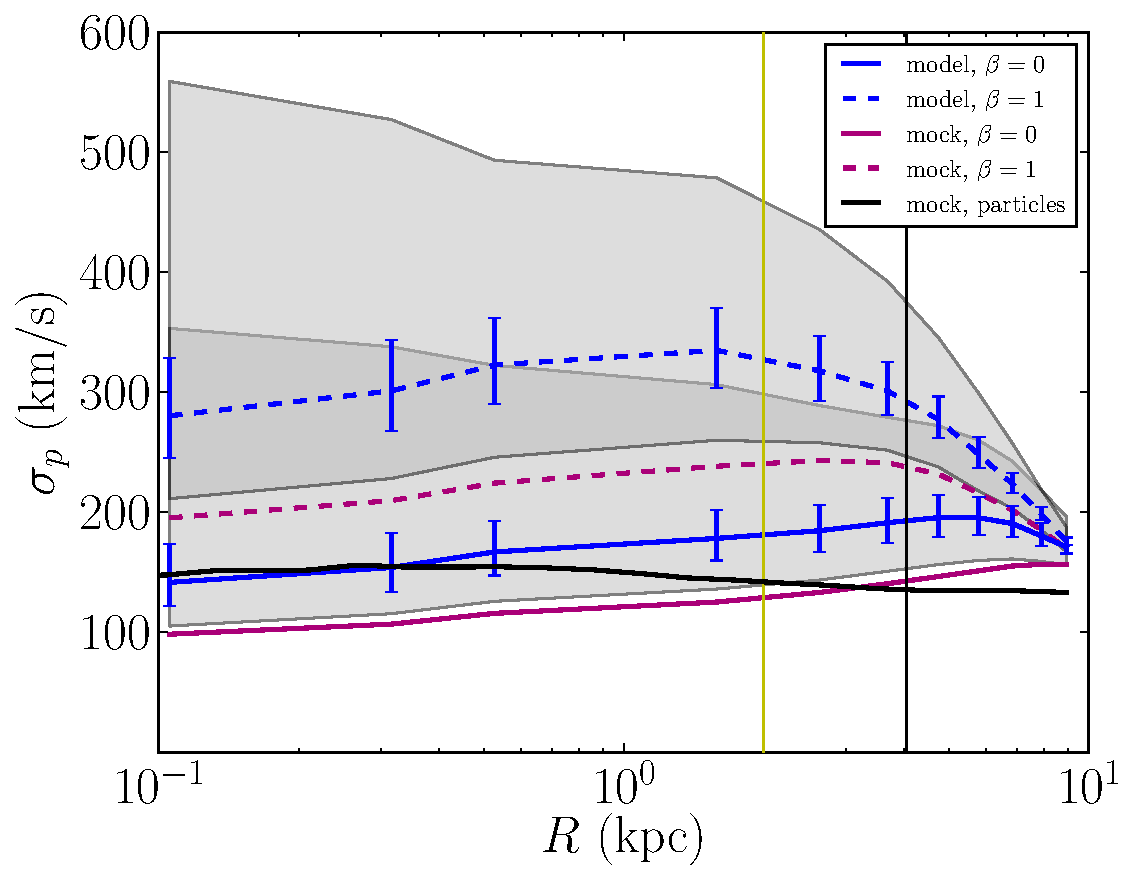
\includegraphics[width=0.33\textwidth]{BCQuadR1a_TmS_sigp-2.pdf}
\caption{
  Estimated projected radially averaged velocity dispersion (\eqnref{eqn:sphericaljeans}) $\sigma_p$ for two Sdom/DMcuspy models ZContrastR1R3
  (left) and QuadR1a (right) assuming an anisotropy $\beta=0$ (blue, solid) and $\beta=1$
  (blue, dashed).  Also shown are the equivalent curves for the mock data after
  running it through the deprojection routines (grey). The solid black line is
  the actual cylindrically averaged velocity dispersion of the original mock particle data.
  The stellar half mass radius (yellow) Einstein
radius (black) are marked by vertical lines. For this configuration, these two
radii are well-separated.}
  \label{fig:sigp} \end{figure*}

\subsection{Stellar mass}
\label{stellar mass}

The stellar mass distribution gives a lower bound on the total mass. Where the stars dominate the central potential, it can provide a powerful constraint extra to the strong lensing data. We took the stellar mass directly from
the generated galaxies and projected the particles onto the pixels. \Glass\
also offers an option to interpolate any map of stellar mass (e.g., from an
observation) onto the pixels. The linear constraint is added to \Glass\ by
writing $\kappa_n = \kappa_{dm,n} + \kappa_{s,n}$ as the sum of the
dark matter and stellar mass components in the potential (\eqnref{discrete
potential}). Since each $\kappa_{s,n}$ is just a constant we do not add new,
separate equations for each pixel. Although we assume a perfect recovery of the stellar mass here, it is straightforward to add errors as the stellar mass constraint remains linear: $\kappa_n = \kappa_{dm,n} + \epsilon \kappa_{s,n}$, where $\epsilon \sim 1$ is an additional error parameter. 

With the stellar mass lower bound, the improvement of the reconstruction
quality shown in \figref{main results} is quite dramatic for the
steepest mock galaxies (AC and BC). This is because these models are dominated
by stars in the inner region. By contrast, the other two galaxies -- where the stars contribute negligibly to the potential -- are unaffected.

\subsection{Stellar kinematics}\label{sec:results_stellar_kinematics}

As outlined in \S\ref{sec:glass}, \Glass\ can also run post processing routines
on the model ensemble which can be used to apply non-linear constraints. As an
example, we consider here constraints from stellar kinematics. The models in
the \Glass\ ensemble are processed as described in \S\ref{sec:glasskinematics}.
To illustrate the power of stellar kinematic constraints, in
\figref{sigma-beta}, we plot the projected velocity dispersion calculated for
one model model (extracted from the full ensemble) of the BC Quad with time
delays and stellar mass (left), and the mean projected velocity dispersion
(\eqnref{eqn:virialaverage}) as a function of the upper limit of the averaging
integral (the aperture size), $a_p$ (right). In both cases, we calculate curves
for two extrema velocity anisotropies: $\beta=0$ (green) and $\beta=1$ (red).
Over-plotted is the correct answer for the BC model (black). The stellar half
mass radius (yellow) Einstein radius (black) are marked by vertical lines. For
this configuration, these two radii are well-separated.

Without even sweeping through the model ensemble and formally
accepting/rejecting models, \figref{sigma-beta} already illustrates what we can
hope to obtain from stellar kinematics. The most robust constraints follow if
we can integrate out the effect of $\beta$ (right panel), since this is
difficult to measure. For large enough aperture size ($a_p > 2r_{1/2}$), the
average projected dispersion converges on a single well defined value
independently of $\beta$. Since this converged value follows from the virial
theorem, it is also rather insensitive to the shape of the potential
\citep{2012ApJ...754L..39A}: it constitutes a robust constraint on the lensing
potential. On the other hand, if the mass profile is well-constrained already
at $r \sim r_{1/2}$, then we can use stellar kinematics to probe $\beta$. This
can be seen in the left panel of \figref{sigma-beta}. Here we see that for a
well-constrained mass model, the $\beta = 1$ curve lies significantly off from
the true answer that has $\beta(r) \sim 0$. 

We now consider formally accepting/rejecting models from the full ensemble. We
consider two regimes of interest: a model with a double where the mass profile
is poorly constrained (XXX), and a model where the mass profile is very well
constrained by the lens data (YYY). In the former case, we use
$\overline{\sigma}(2 r_{1/2})$ to probe the mass independently of $\beta(r)$.
We accept/reject models assuming a Gaussian error on measured
$\overline{\sigma}(2 r_{1/2})$ of $\pm 10$\,km/s (similarly to the data quality
presented for example in \citealt{2002MNRAS.337L...6T}). The results are shown
in \figref{main results}, blue data points. In the latter case, we ask whether
the data favour $\beta = 0$ or $\beta = 1$ by obtaining a $\chi^2$ goodness of
fit measure between the true and modelled $\sigma_p(R)$. We accept/reject
models from the ensemble above. The results for $\beta$ are shown in Figure
ZZZ. 

The results for stellar kinematics match our expectations from
\S\ref{sec:kinematics}. Where the lens data already constrain the mass
distribution at $r \sim r_{1/2}$, stellar kinematics provide valuable
information about the velocity anisotropy of the stars, $\beta$ (see Figure
ZZZ). Where the lens data poorly constrain the mass distribution at $r_{1/2}$,
we may `integrate out' the effect of unknown $\beta$ to obtain a robust measure
of $M(r_{1/2})$ from the stellar kinematics. This latter is robust to both
uncertainties in $\beta(r)$ and to our assumption of spherical symmetry in the
kinematic models \citep{2012ApJ...754L..39A}. Finally, we note that there is a
third interesting case. If the lens models well-constrain $M(r_{1/2})$ and
stellar kinematics are available, then these can be used to probe cosmological
models (see \S\ref{sec:theory}). We explore this in more detail in a separate
publication. 

%\begin{figure*}
%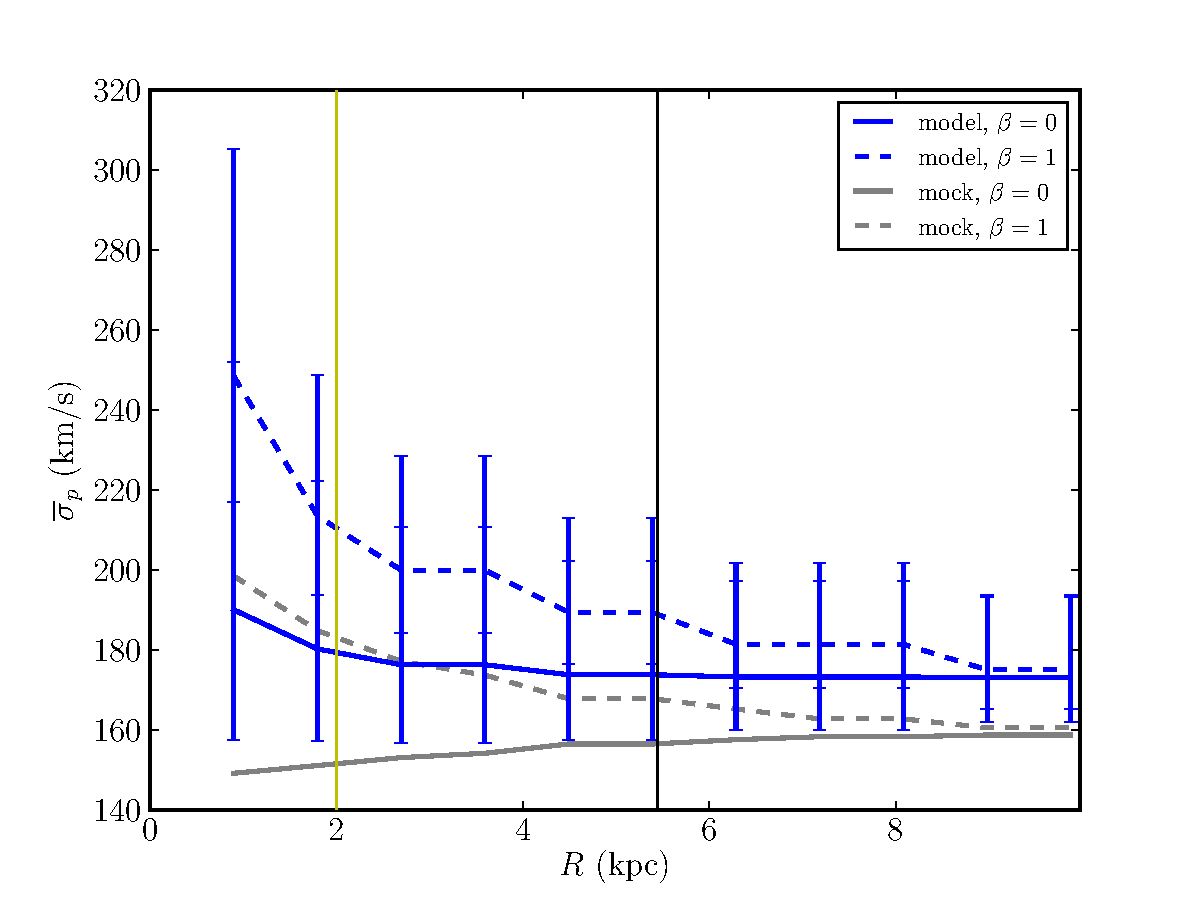
\includegraphics[width=0.49\textwidth]{BCQuadR1a_TmS_sigpbar.pdf}
%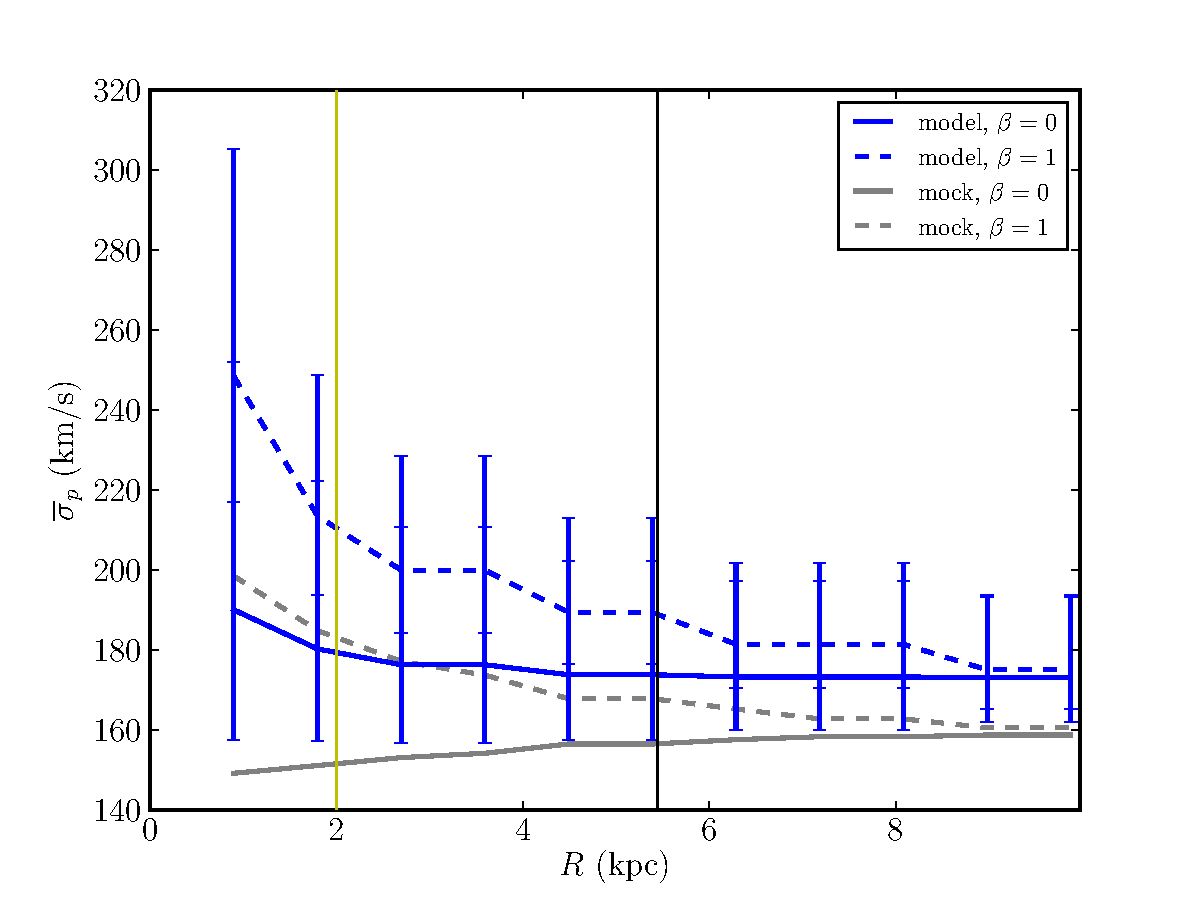
\includegraphics[width=0.49\textwidth]{BCQuadR1a_TmS_sigpbar.pdf}
%\caption{{\bf Left:} 
%The mean projected velocity dispersion (\eqnref{eqn:virialaverage}) as a function of the upper
%limit of the averaging integral (the aperture size), $a_p$
%  for two Sdom/DMcuspy models ZContrastR1R3
%  (left) and QuadR1a (right) assuming two extrema velocity anisotropies $\beta=0$ (blue, solid) and $\beta=1$
%  (blue, dashed).  Also shown are the equivalent curves for the mock data after
%  running it through the deprojection routines (grey). 
%\sout{Over-plotted is the correct answer for the BC model (black)
%  {\bf JR. Jonathan to add}.} 
%  The stellar half mass radius (yellow) Einstein
%radius (black) are marked by vertical lines. For this configuration, these two
%radii are well-separated.}
%\label{sigma-beta}
%\end{figure*}

%\subsection{Velocity dispersions}
%
%\begin{itemize}
%\item Can they predict radial profiles?
%\item Can we constrain lensing models from predicted velocity dispersions?
%\item Use a constructed spherical halo G2 following a $\rho \propto r^{-\gamma}$ profile with stellar halo same as G1.
%\item Vary $z$ of the halo, possibly orientation.
%\item Should be able to recover $\gamma$ very well.
%\item Use G1. Show problems with recovering $\gamma$.
%\end{itemize}

%\subsection{With/without time delays and central image} %--------------------------------------------------------------

%We also considered the effect of having time delays or a central image. The
%central image is usually highly demagnified and obscured by the lensing galaxy,
%but in clusters the central image is observable. In this case we can imagine
%the galaxies to be clusters since the problem is scale-free. A recontruction of
%AASingleQuadR1a\_Tm is shown in \figref{AASingleQuadR1a_Tm}. The suffix denotes
%which combination of time delays (T) and central image (M) was used. An
%uppercase letter indicates the feature is turned on, and a lowercase letter
%that it is turned off.

\section{Conclusions}\label{sec:conclusions}

Various action items.

\subsection{Goodness of recovery}

\begin{enumerate}

  \item \sout{Change variable $\chi$ to something else ($f$?) to avoid confusion with $\chi^2$.}

  \item \sout{Correct equation \eqref{badness} to describe what is actually calculated.}

  \item \sout{Show results for $1\sigma$ and $2\sigma$ rather than full \Glass\ ensemble.}

\item Add results for Claudio's shape measure. Discuss shape
  throughout results section and mention more explicitly in abstract
  and conclusions -- what quality of data do we need to robustly
  constrain the shape?

\item Add plot of $\chi$ ($f$) for $lambda_1/lambda_2$ and shape
  parameters (cf. what Claudio is doing).

\item \sout{Check that you and Claudio average to the same projected radius
  (one pixel past outermost image) when calculating
  $lambda_1/lambda_2$ and $\theta$.}. This is correct.

\end{enumerate}

\subsection{Kinematics}

\begin{enumerate}

\item \sout{Add example plot of the projected density and recovered
  projected density (cf. plots Jonathan made for Justin's ERC
proposal).}

\item Calculate aperture averaged $\sigma$ to 2 (or 3 you decide) half
  light radii assuming $\beta = 0$ for a model (double) where the mass
  is poorly constrained by strong lensing. Accept/reject models from
  the ensemble $\Longrightarrow$ what we learn from combined lensing
  kinematics.

\item \sout{Take a model that is well constrained by strong lensing
  (e.g. quad with time delays). Calculate $\sigma_p(R)$ for each model
  in the ensemble using the kinematics module. Compare this with the
true $\sigma_p(R)$ from the mock data to obtain a $\chi^2$ (actually
  a $\chi^2$ this time!). Show the true $\sigma_p(R)$ and overlay
  coloured bands from the lensing model ensemble assuming $\beta = 0$
or $\beta = 1$.}

\item Add accept/reject results for stellar kinematics (two figures)
  as detailed in \S\ref{sec:results_stellar_kinematics}.

\end{enumerate}

\subsection{Other}

\begin{enumerate}

\item Tidy up figures and other small items as detailed throughout --
  see {\bf JR ... }

\item Add appendix showing how inversion symmetry in the prior affects
  results. Clarify meaning of this prior with a nice figure showing
  the symmetry.

\item Complete \S\ref{sec:glass}. Emphasise need for central adaptive
  grid. Add appendix showing convergence as Pixrad is increased.

\end{enumerate}

\subsection{Clarifications in text}

\begin{enumerate} 

\item Write section \S\ref{sec:glassextraimages} on removing models
  with extra images.

\item Clarify amount of triaxiality (and the analytic density profile)
  in \S\ref{sec:mockdata}.

\item \sout{Clarify number of lens configurations in \S\ref{sec:lensconfig}.}

\end{enumerate}


\appendix

\section{Implementation Details}

Since we want to model the density distribution with a computer it
is convenient to choose units that make the relevant quantities of order
unity.  We therefore measure lengths in light years, time in years, positions
in arcseconds, and choose $c=1$ and $4\pi G = N^2$, where $N^2 \equiv 206,265$
arcsec/rad. The mass unit is then $11.988\ \Msun$. It will also be useful to
define a proxy to the Hubble constant $\zeta \equiv N^2 H_0$. We now 
express the equations from \secref{sec:theory} in terms of these new units
and introduce some other useful quantities.

The lens equation in its complete form becomes:
%
\begin{eqnarray}
N^2ct(\vec\theta) & = & (1+z_L)\frac{D_{L}D_{S}}{D_{LS}}\frac12 |\vec\theta - \vec\beta|^2 \nonumber \\
& & - (1+z_L)\frac{4GD_{L}^2}{c^2}\int \Sigma(\vec\theta') \ln |\vec\theta-\vec\theta'| d^2\vec\theta'
\label{eqn:full_arrival_time}
\end{eqnarray}
%
where the factor of $D_L^2$ in the second term comes from the fact that $\Sigma$
has units of \Msun/lyr$^2$. We can clean this up by first writing down a dimensionless time
delay
%
\begin{equation}
\tau = \left[ (1+z_L) d_L\right]^{-1}\zeta t
\label{tau}
\end{equation}
%
in terms of our previous definitions and defining $D_L \equiv (c/H_0)d_L$. We
further define a dimensionless density
%
\begin{equation}
\kappa_\infty = \frac{4\pi G}{c^2}\frac{c}{H_0}d_L\Sigma
              = \frac{d_L}{\zeta}\Sigma
\end{equation}
%
and a lensing potential
%
\begin{equation}
\psi(\vec\theta) = \frac1\pi \int \kappa_\infty(\vec\theta') \ln|\vec\theta - \vec\theta'| d^2\vec\theta'\
\label{lensing potential}
\end{equation}
%
Now we can express \eqnref{eqn:full_arrival_time} very compactly as
%
\begin{equation}
\tau(\vec\theta) = \frac12 \xi |\vec\theta-\vec\beta|^2 - \psi(\vec\theta)
\label{arrival time}
\end{equation}
%
where $\xi=d_S / d_{LS}$.
We explicitly write $\kappa_\infty$ to remind ourselves
that there is no source distance factor involved. This is useful when we
consider multiple sources.

\section{Raytracing convergence test}
Raytracing is sensitive to the map area and resolution set by $\Rmap$ and
$\Rpix$.  In the left panel of \figref{raytracing convergence tests} we compare
the change in time delays as we increase $\Rmap$.  The image system is a quad
with the central maximum image. When the projected mass begins to fall off the
time delays stabilize. In the right panel we see the effect of changing the
resolution of the map.  Increasing the resolution allows for more accurate
placement of the images and after about $\Rpix=40$ the image positions change
by less than 0.04 arcsec. The one image that continues to change is near to a
caustic.  

\begin{figure}
\plottwo{tdconv_pr45.pdf}{imgpos_conv_mr20.pdf}
\caption{(left) Test for predicted time delay convergence as $\Rmap$ changes.
$\Rpix=45$. After about $\Rmap=20$ most of the asymmetric mass is in the map.
(right) Test for predicted image position $\theta$ convergence as $\Rpix$
changes. $\Rmap=20$ arcsec.}
\label{raytracing convergence tests}
\end{figure}

\section{Derivation of pixelated density coefficients}
\label{Q derivation}
When the lens plane is pixelized we need a discrete form of the integral
%
\[\int \kappa(\vec\theta') \ln |\vec\theta-\vec\theta'| d^2\vec\theta' \]
%
In particular we want
%
\[\sum_n \kappa_n Q_n(\vec\theta)\]
%
where $Q_n$ is the logarithm evaluated over the $n$th pixel at position $\vec\theta_n = (x_n, y_n)$. Let the pixel side length be $a$.
Instead of working with a position vector $\vec\theta$ we work in cartesian coordinates where 
%
$|\vec\theta| = r = \sqrt{x^2 + y^2}$. The integral now becomes
%
\[Q_n(x,y) = \frac12 \int_{y_-}^{y_+}\int_{x_-}^{x_+} \ln (x'^2+y'^2) dx' dy'\]
%
where $x_\pm = x + x_n \pm (a/2)$ and similarly for $y_\pm$.
Using the identity
%
\[\int \ln(x^2+y^2) dx = x \ln(x^2+y^2) - 2x + 2y\arctan(x/a) \]
%
we can express $Q_n$ as the sum of four parts
%
\begin{align*}
Q_n(x,y) = \frac12 [\tilde Q_n(x_+,y_+)
                  + \tilde Q_n(x_-,y_-) & 
\\                - \tilde Q_n(x_-,y_+)
                  - \tilde Q_n(x_+,y_-) ]
\end{align*}
%
where
%
\[\tilde Q_n(x,y) = xy(\ln r^2 - 3) + x^2\arctan(y/x) + y^2\arctan(x/y)\]

\section{Pixel resolution convergence test}
{\bf JR. Need to add an appendix showing convergence with increasing Pixrad.} 

\bibliographystyle{mn2e}
\bibliography{ms}

\end{document}

\cite{2007ApJ...667..645R} were the first to test the recovery of
strong lensing surface density profiles using mock data generated from
N-body models {\bf JR. Is this true?}. They found that when including
time delays, circularly averaged surface density distributions can
sufficiently well-recovered to make interesting comparisons with
theoretical models Cosmological parameters, however, are more
sensitive. Since then, several groups have used N-body mock data to
explore the fidelity of strong lensing reconstructions
\citep{2007MNRAS.380.1729L}. We expand on these earlier works
by considering not only the recovery of the circularly averaged
surface density profile of a lens, but also its shape, higher order
measures of the mass recovery (a pixel-by-pixel comparison), and the
utility of wrapping in constraints from stellar mass estimates and/or
stellar kinematics.




